%%%%%%%%%%%%%%%%%%%%%%%%%%%%%%%%%%%%%%%%%%  不使用 authblk 包制作标题  %%%%%%%%%%%%%%%%%%%%%%%%%%%%%%%%%%%%%%%%%%%%%%
%-------------------------------PPT Title-------------------------------------
\title{量子计算、量子通信和量子加密}
%\subtitle{两弹元勋与核弹原理}
%-----------------------------------------------------------------------------

%----------------------------Author & Date------------------------------------
%\author[]{\vskip +10pt 高朋林\inst{}} %[]{} (optional, use only with lots of authors)
%% - Give the names in the same order as the appear in the paper.
%% - Use the \inst{?} command only if the authors have different
%%   affiliation.
\institute[BCC]{\inst{}%
%\institute[Gain~Strong]{\inst{}%
\vskip -15pt 北京市计算中心}
%\vskip -20pt {\large 格致斯创~科技}}
\date[\today] % (optional, should be abbreviation of conference name)
{	%{\fontsize{6.2pt}{4.2pt}\selectfont{\textcolor{blue}{E-mail:~}\url{jiangjun@bcc.ac.cn}}}
\vskip 45 pt {\fontsize{8.2pt}{6.2pt}\selectfont{%清华大学\;\;物理系% 报告地点
	\vskip 5 pt \textrm{2025.04}}}
}

%% - Either use conference name or its abbreviation
%% - Not really information to the audience, more for people (including
%%   yourself) who are reading the slides onlin%%   yourself) who are reading the slides onlin%%   yourself) who are reading the slides onlineee
%%%%%%%%%%%%%%%%%%%%%%%%%%%%%%%%%%%%%%%%%%%%%%%%%%%%%%%%%%%%%%%%%%%%%%%%%%%%%%%%%%%%%%%%%%%%%%%%%%%%%%%%%%%%%%%%%%%%%

\subject{}
% This is only inserted into the PDF information catalog. Can be left
% out.
%\maketitle
\frame
{
%	\frametitle{\fontsize{9.5pt}{5.2pt}\selectfont{\textcolor{orange}{“高通量并发式材料计算算法与软件”年度检查}}}
\titlepage
}
%-----------------------------------------------------------------------------

%------------------------------------------------------------------------------列出全文 outline ---------------------------------------------------------------------------------
\section*{}
\frame[allowframebreaks]
{
	\frametitle{\textrm{Outline}}
%  \frametitle{\textcolor{mycolor}{\secname}}
  \tableofcontents%[current,currentsection,currentsubsection]
}
%在每个section之前列出全部Outline
%类似的在每个subsection之前列出全部Outline是\AtBeginSubsection[]
%\AtBeginSection[]
%{
%  \frame<handout:0>%[allowframebreaks]
%  {
%    \frametitle{Outline}
%%全部Outline中,本部分加亮
%    \tableofcontents[current,currentsection]
%  }
%}

%-----------------------------------------------PPT main Body------------------------------------------------------------------------------------
% 量子相干态部分
\section{量子相干态}
\begin{frame}
    \frametitle{量子相干态简介}
    \begin{itemize}
	    \item 在经典物理中,物体的状态是确定的;~而量子系统中可以存在多个量子态叠加的量子相干\textrm{(Coherent)}态
            \begin{figure}
        \centering
                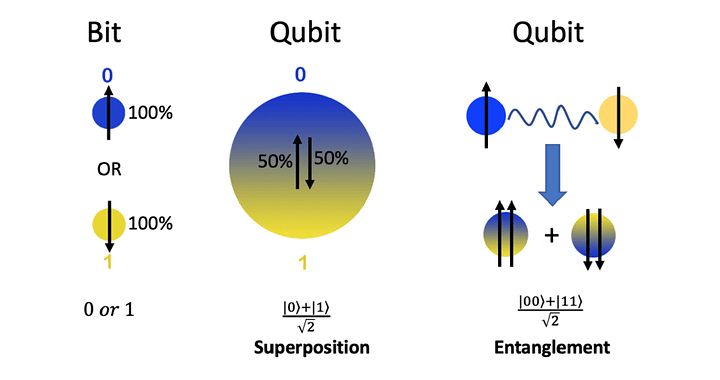
\includegraphics[height=0.7in, width=1.0in, viewport=0 0 460 330,clip]{Figures/Illustration-of-a-bit_and_qubit.png}
		\hspace{0.1in}
                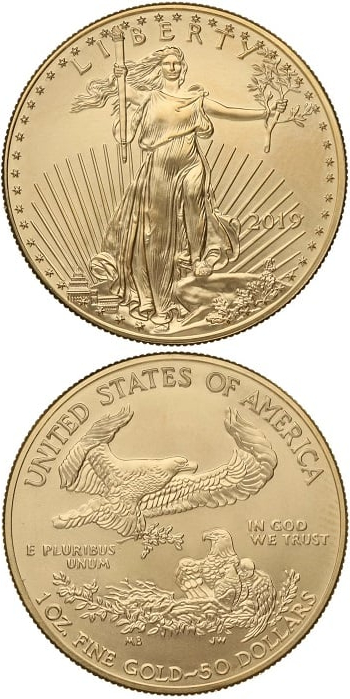
\includegraphics[height=0.7in, width=0.35in, viewport=0 0 85 170,clip]{Figures/American_Eagle_gold_coin_2019_2.jpg}
                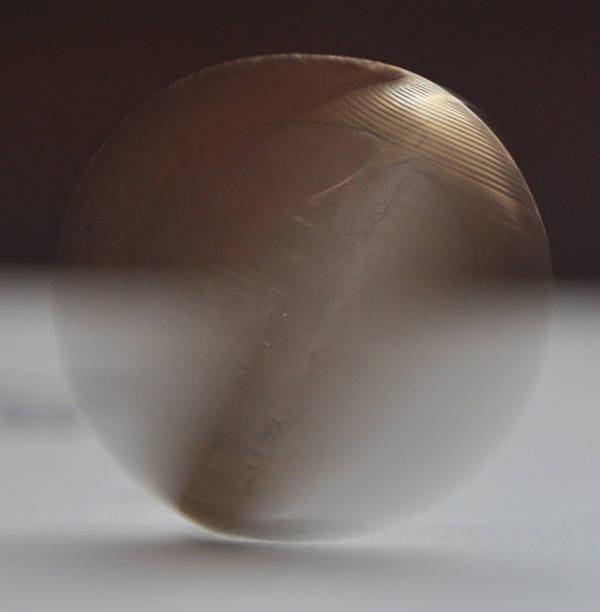
\includegraphics[height=0.7in, width=0.7in, viewport=0 0 150 151,clip]{Figures/Coin-spin.jpg}
%                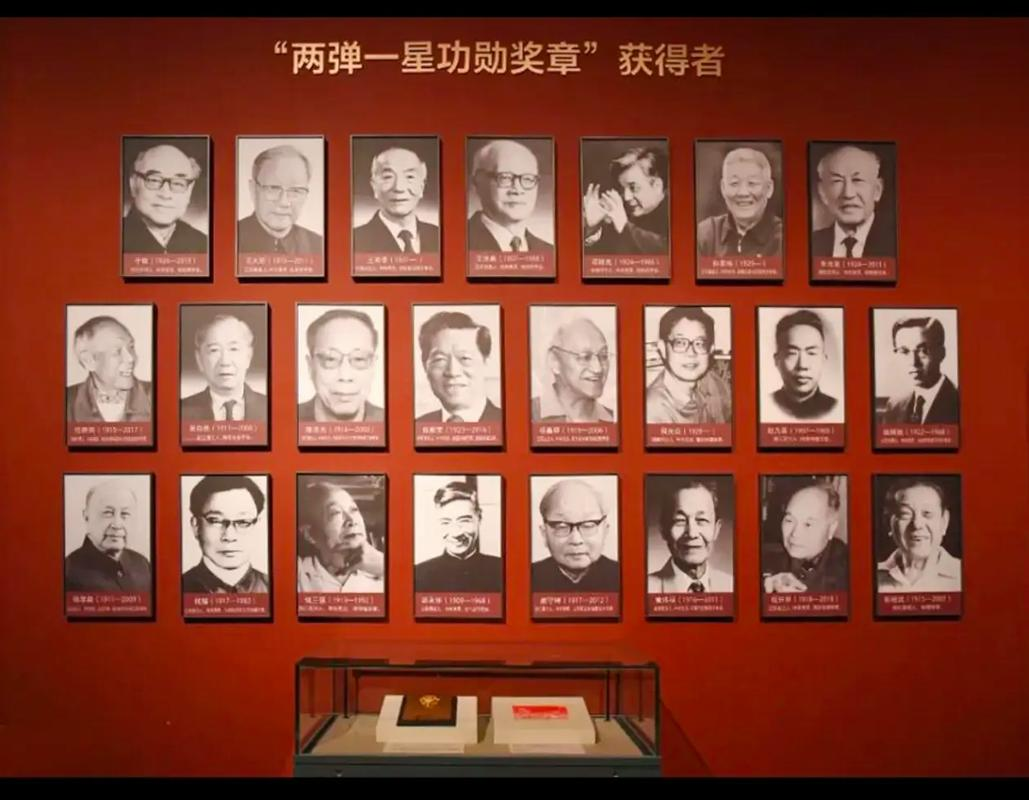
\includegraphics[width=0.95\textwidth]{Figures_History/Collection_23-1.jpeg}
		\caption{\tiny{\textrm{Schematic diagram of coherence of particle.}}}
		\label{Fig:Schematic-Coherence-of-particle}
            \end{figure}
	    \vskip -0.24in
	    {\fontsize{8.5pt}{5.2pt}\selectfont{\textcolor{magenta}{叠加态之间存在确定的相位关系}}}
        \item 量子相干使得粒子可以同时处于多个状态
            \begin{figure}
        \centering
%                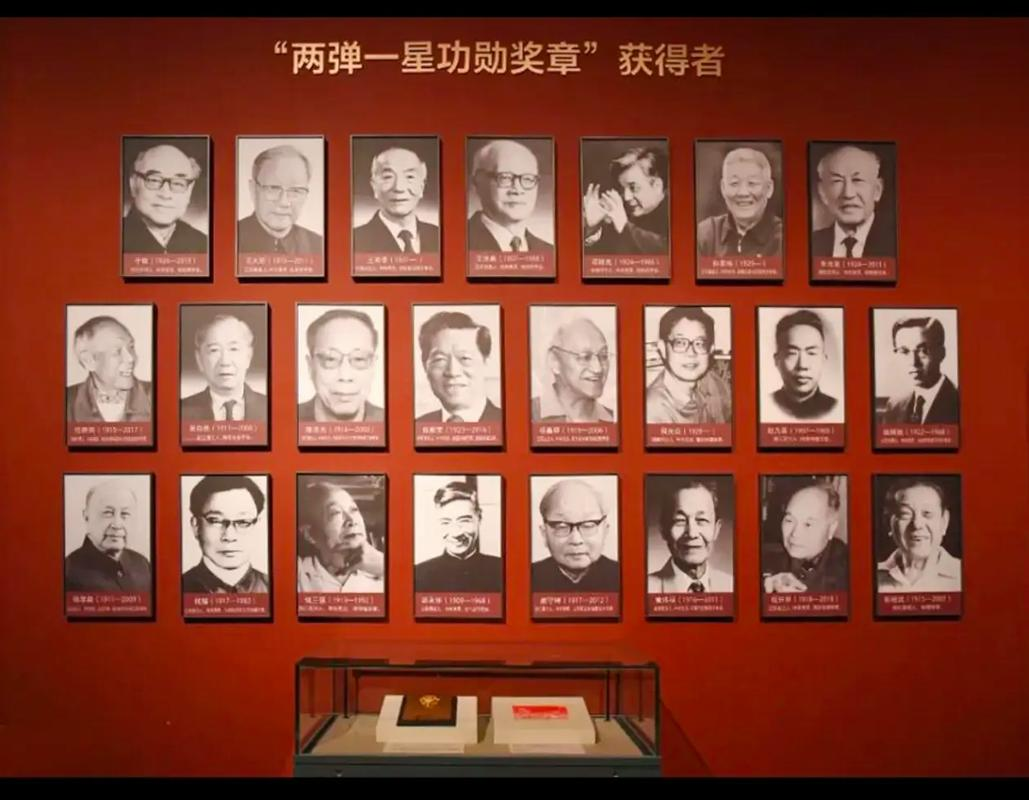
\includegraphics[width=0.95\textwidth]{Figures_History/Collection_23-1.jpeg}
                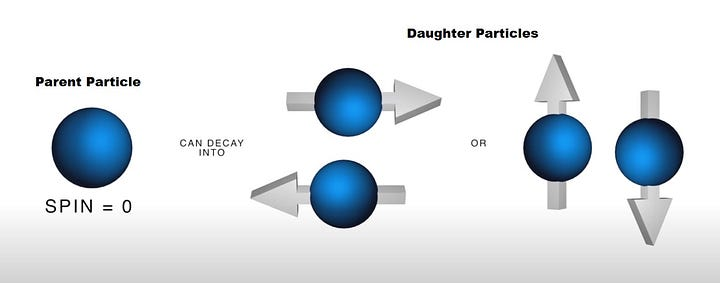
\includegraphics[height=0.8in, width=2.2in, viewport=0 0 720 283,clip]{Figures/Schematic-Coherence-of-particle.jpeg}
		\caption{\tiny{\textrm{Illustration of the decay of a quantum coherent state.}}}
		\label{Fig:Illustration-of-a-bit_and_qubit}
            \end{figure}
    \end{itemize}
\end{frame}

\begin{frame}
    \frametitle{量子相干态的重要性}
    \textcolor{magenta}{量子相干态:~量子计算和量子通信的基础}
    \begin{itemize}
        \item {\fontsize{8.5pt}{5.2pt}\selectfont{量子计算:~并行计算正是利用相干态的叠加特性实现的}}
	\item {\fontsize{8.5pt}{5.2pt}\selectfont{量子信息处理:~相干态的保持可确保信息的准确传输和处理}}
    \end{itemize}
{\fontsize{7.5pt}{5.2pt}\selectfont{
    \begin{exampleblock}{示例:~量子比特的相干态}
        一个量子比特可以处于 \( |0\rangle \) 和 \( |1\rangle \) 的相干叠加态 \( \alpha|0\rangle+\beta|1\rangle \),其中 \( |\alpha|^2 + |\beta|^2 = 1 \)
\end{exampleblock}}}
            \begin{figure}
        \centering
                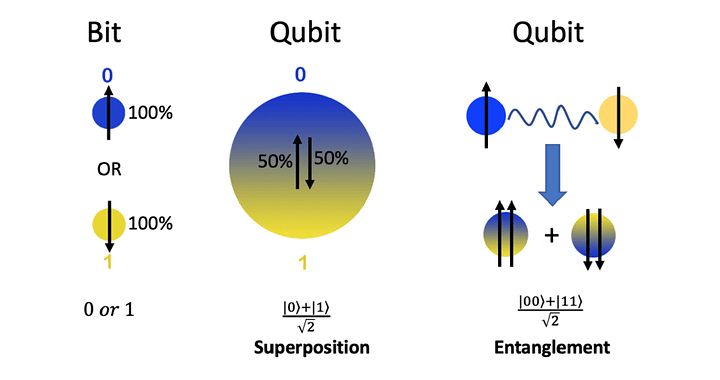
\includegraphics[height=1.5in, width=2.0in, viewport=0 0 460 380,clip]{Figures/Illustration-of-a-bit_and_qubit.png}
%                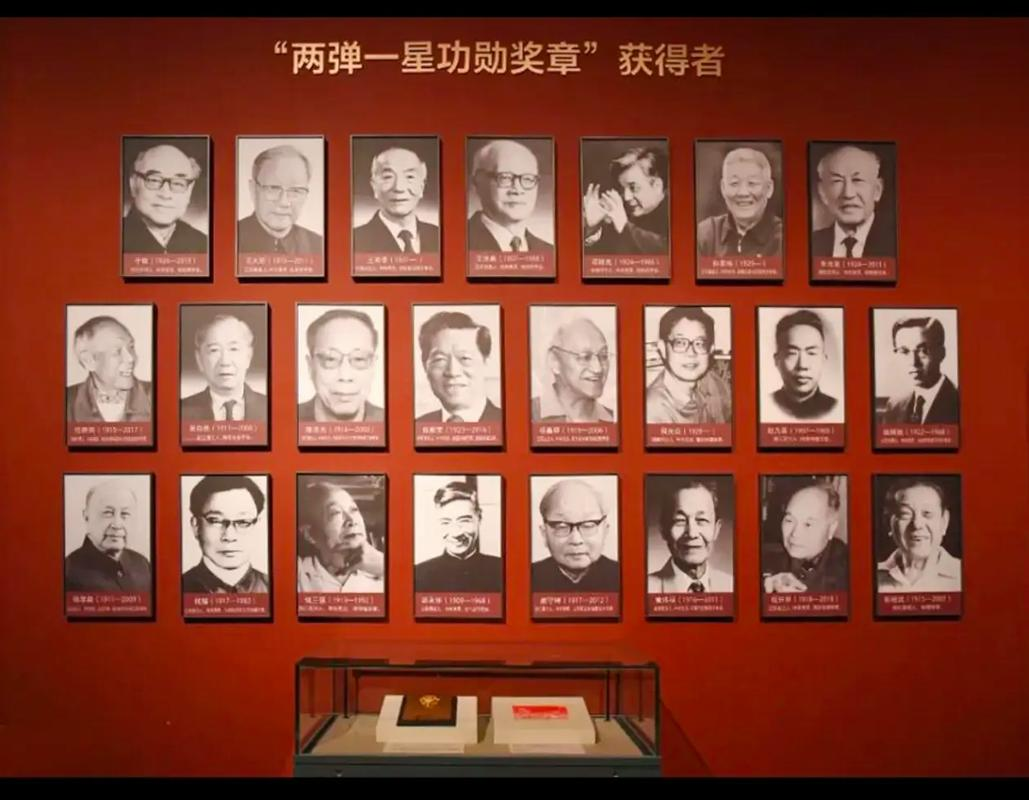
\includegraphics[width=0.95\textwidth]{Figures_History/Collection_23-1.jpeg}
		\caption{\tiny{\textrm{Schematic diagram of a qubite.}}}
		\label{Fig:Schematic-Coherence-of-particle_2}
            \end{figure}
\end{frame}

\begin{frame}
    \frametitle{量子相干态的挑战:~退相干}
        当量子系统与外界环境相互作用时,相干态会受到破坏,该过程称为退相干
            \begin{figure}
        \centering
                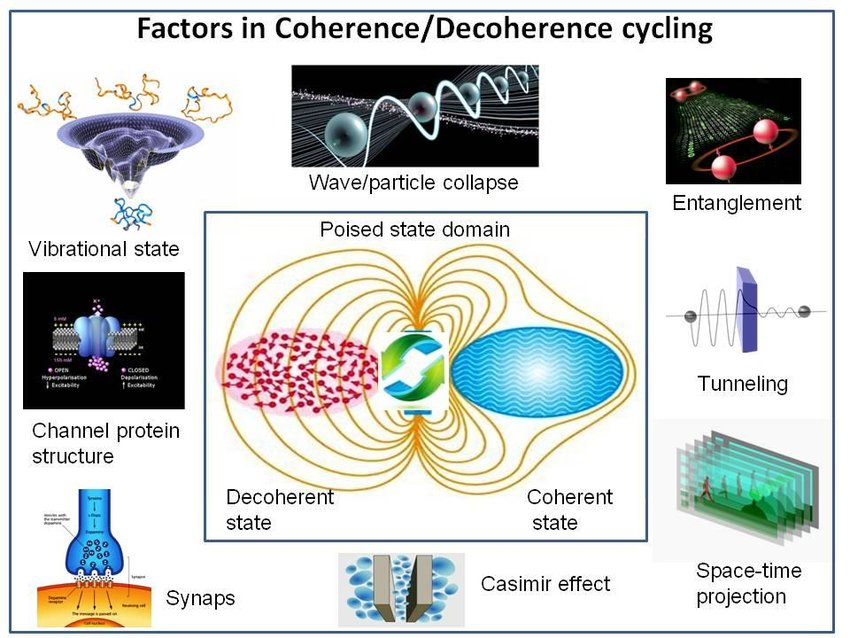
\includegraphics[height=1.3in, width=1.7in, viewport=0 0 650 470,clip]{Figures/Schematic-representation-of-a-poised-realm-allowing-coherence-and-de-coherence-cycles.jpeg}
%                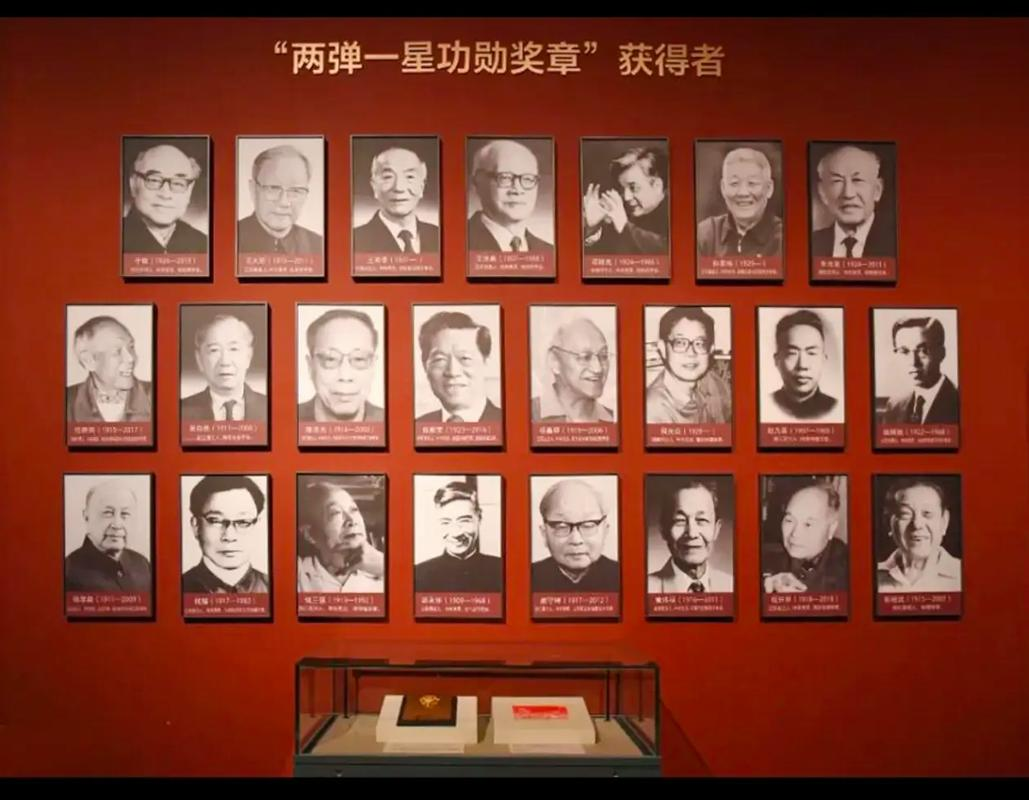
\includegraphics[width=0.95\textwidth]{Figures_History/Collection_23-1.jpeg}
		\caption{\tiny{\textrm{Schematic representation of a poised realm allowing coherence and de-coherence cycles.}}}
		\label{Fig:Schematic-representation-of-a-poised-realm-allowing-coherence-and-de-coherence-cycles}
            \end{figure}
	    \vskip -10pt
	{\fontsize{9.5pt}{5.2pt}\selectfont{\textcolor{magenta}{退相干是实现大规模量子计算和长距离量子通信的主要障碍}}}
{\fontsize{8.5pt}{5.2pt}\selectfont{
    \begin{alertblock}{应对策略}
        目前采用量子纠错码、量子绝热演化等技术来尽量减少退相干的影响
\end{alertblock}}}
\end{frame}

% 量子计算机基本原理部分
\section{量子计算的基本原理}
\begin{frame}
    \frametitle{量子比特}
    \begin{itemize}
	    \item 经典计算机使用比特\textrm{(bit)}作为信息载体,取值为 0 或 1
	    \item 量子计算机使用量子比特\textrm{(qubit)},可以处于 \( |0\rangle \)、 \( |1\rangle \) 以及它们的任意叠加态 
		    \begin{displaymath}
			    \alpha|0\rangle+\beta|1\rangle
		    \end{displaymath}
		    {\fontsize{7.5pt}{5.2pt}\selectfont{其中 \( \alpha \) 和 \( \beta \) 是复数,且 \( |\alpha|^2 + |\beta|^2 = 1 \)}}
    \end{itemize}
            \begin{figure}
        \centering
                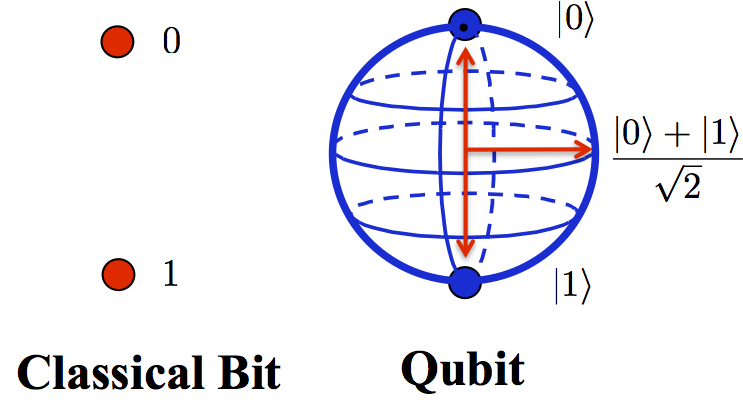
\includegraphics[height=1.5in, width=2.7in, viewport=0 0 360 195,clip]{Figures/Quantum-Bit.png}
%                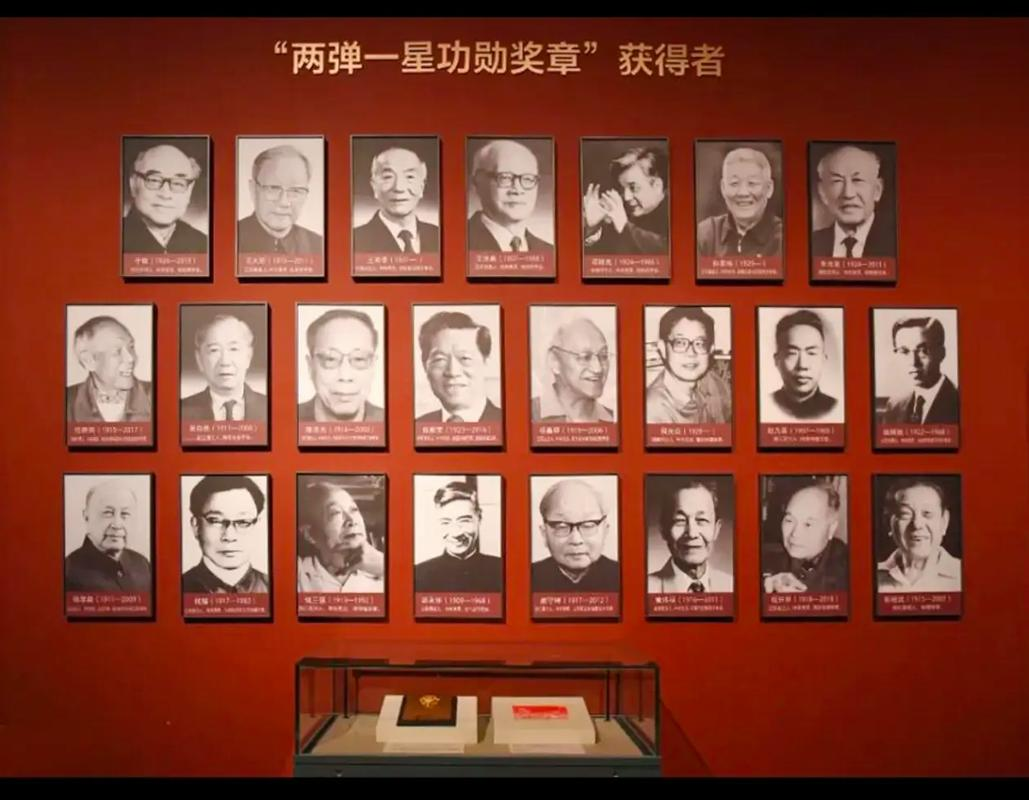
\includegraphics[width=0.95\textwidth]{Figures_History/Collection_23-1.jpeg}
		\caption{\tiny{\textrm{Schematic diagram of a class bit vs qubit.}}}
		\label{Fig:Quantum-Bit}
            \end{figure}
\end{frame}

\begin{frame}
    \frametitle{量子比特与并行}
        量子比特的叠加特性允许其同时处于多个状态:
            \begin{figure}
        \centering
                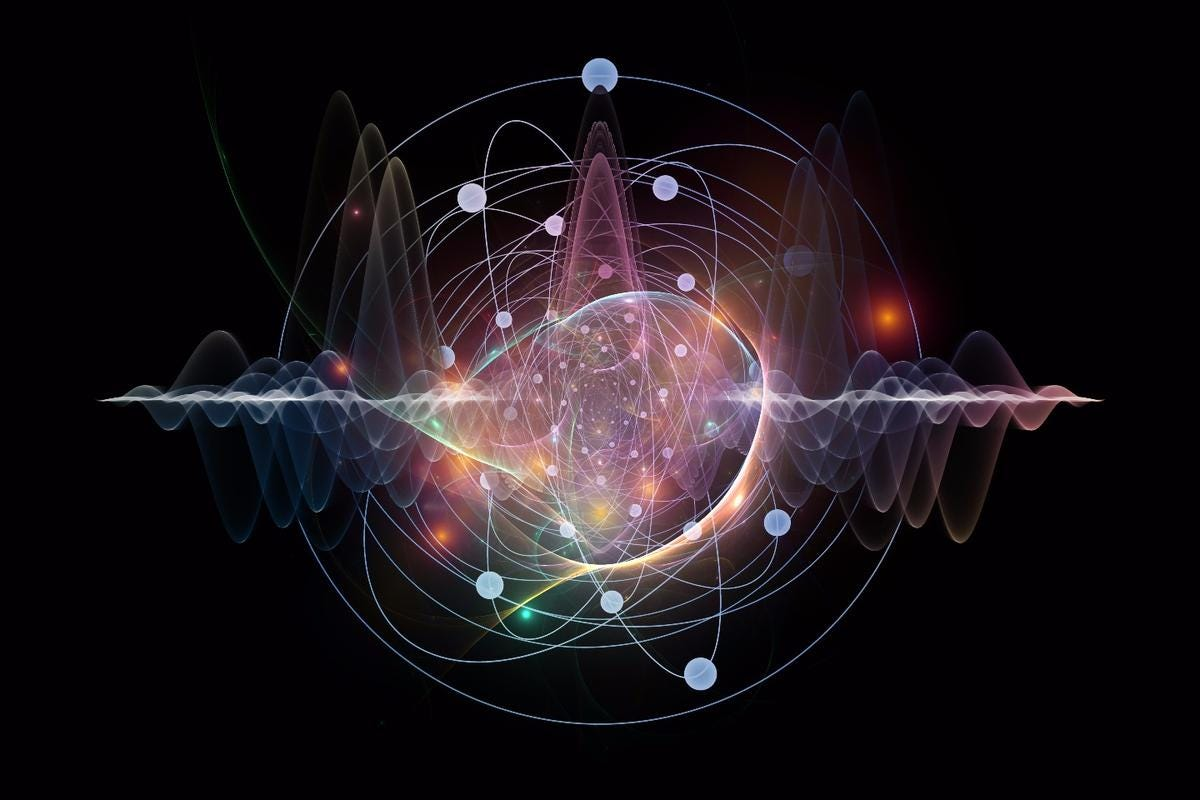
\includegraphics[height=1.0in, width=1.5in, viewport=0 0 1200 800,clip]{Figures/Quantum_Computing_2.jpg}
%                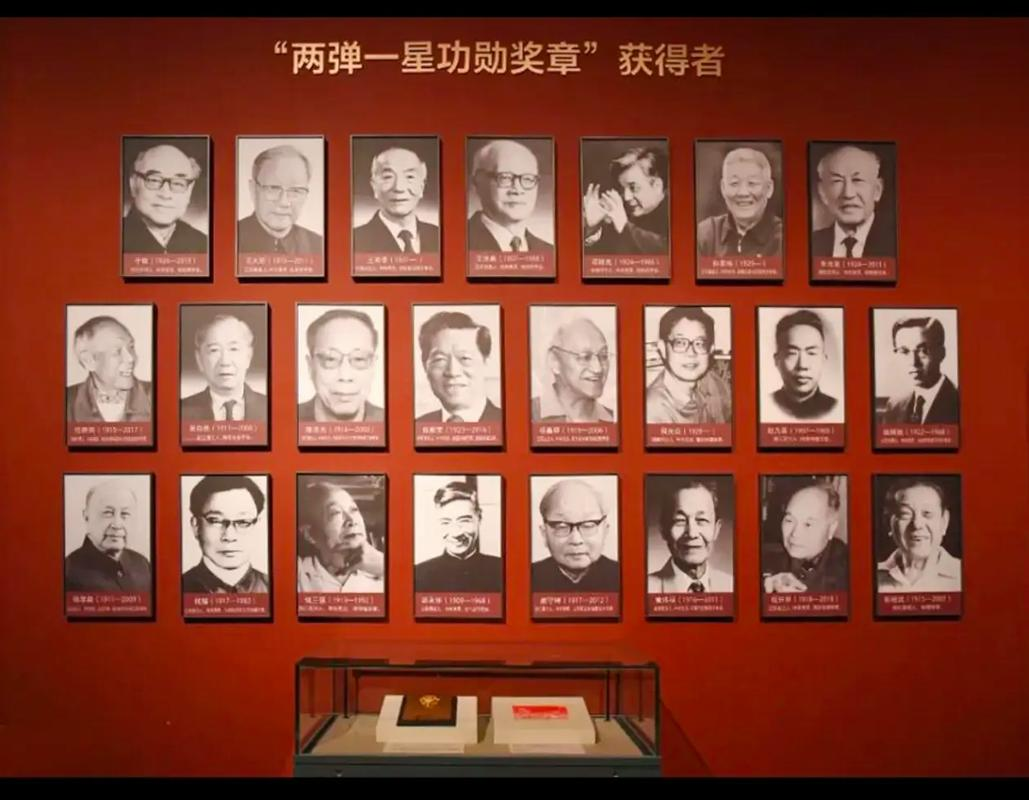
\includegraphics[width=0.95\textwidth]{Figures_History/Collection_23-1.jpeg}
		\caption{\tiny{\textrm{Illustration of the superposition of qubit.}}}
		\label{Fig:Quantum_Computing_2}
            \end{figure}
	    \vskip -15pt
    {\fontsize{7.5pt}{5.2pt}\selectfont{\begin{exampleblock}{示例}
	    \textrm{2} 个量子比特可以同时处于 \( |00\rangle \)、 \( |01\rangle \)、 \( |10\rangle \)、 \( |11\rangle \) 的叠加态 \( \alpha_{00}|00\rangle+\alpha_{01}|01\rangle+\alpha_{10}|10\rangle+\alpha_{11}|11\rangle \)
    \end{exampleblock}}}
    \vskip 2pt
	\textcolor{blue}{\textrm{n} 个量子比特可以同时处于 \( 2^n \) 个状态的叠加}\\
    {\fontsize{9.5pt}{5.2pt}\selectfont{\textcolor{red}{这使得量子计算机在一次操作中可以对 \( 2^n \) 个数据进行计算,实现并行计算,大大提高计算效率}}}
\end{frame}

\begin{frame}
    \frametitle{量子计算的优势}
    \begin{itemize}
        \item 并行计算能力:~可以同时处理多个计算任务\\
		{\fontsize{7.5pt}{5.2pt}\selectfont{\textcolor{blue}{得益于量子相干态的叠加特性}}}
        \item 解决复杂问题:~如大数分解、优化问题等
    \end{itemize}
{\fontsize{7.5pt}{5.2pt}\selectfont{
	\begin{exampleblock}{示例:~\textrm{Shor} 算法}
            \begin{figure}
        \centering
                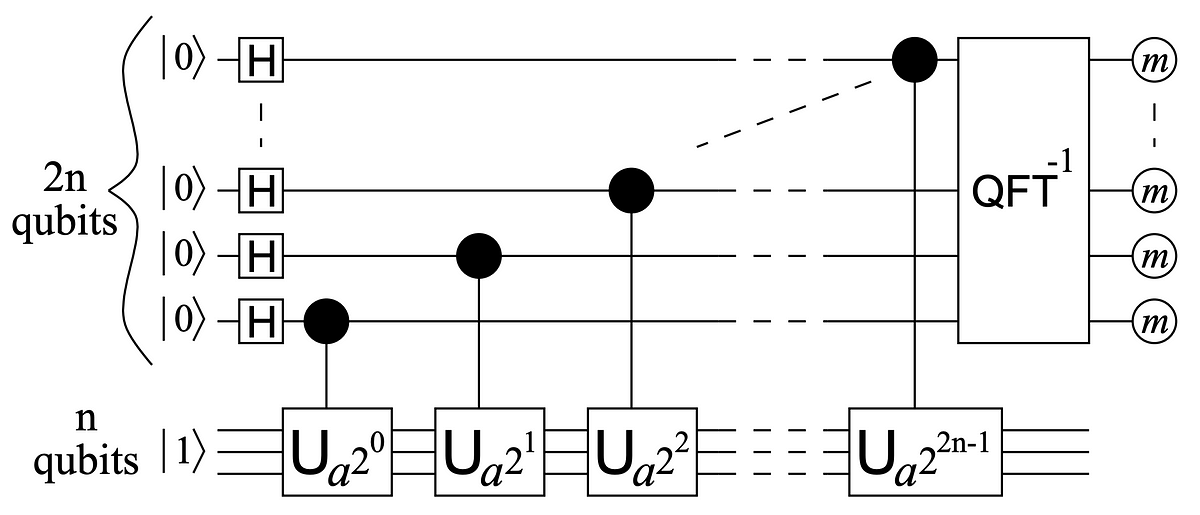
\includegraphics[height=1.0in, width=2.2in, viewport=0 0 1200 515,clip]{Figures/General-implementation-of-shors_algorithm.png}
%                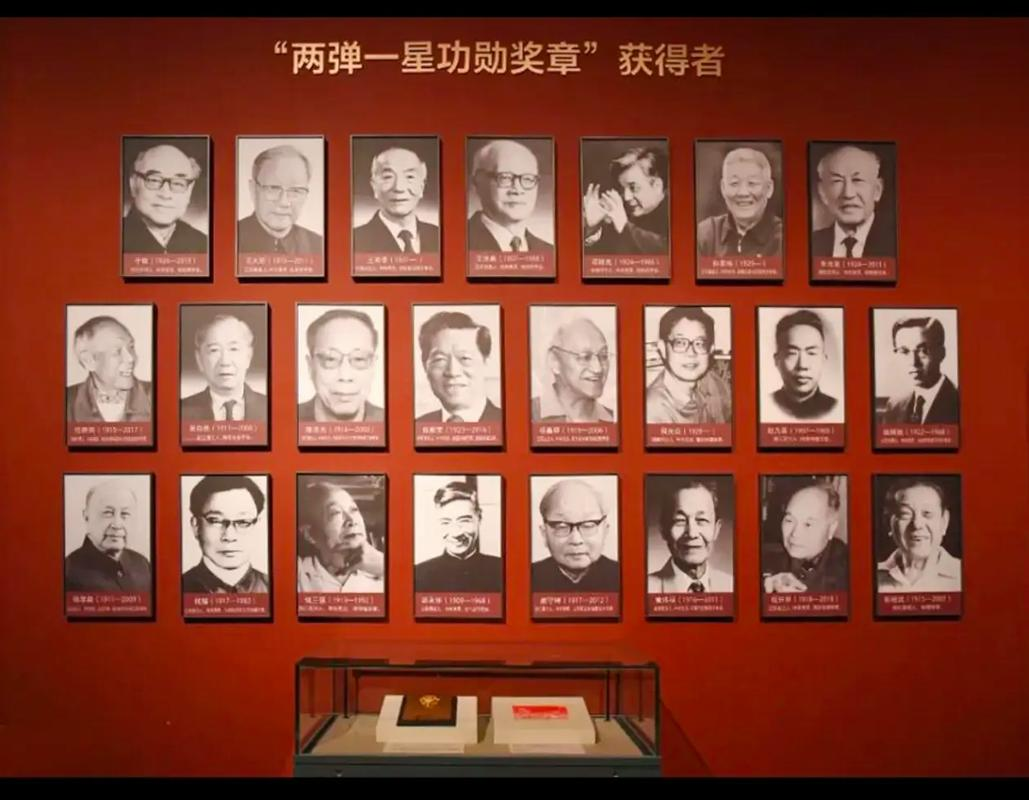
\includegraphics[width=0.95\textwidth]{Figures_History/Collection_23-1.jpeg}
		\caption{\tiny{\textrm{A Schematic illustration of general Order Finding Algorithm.}}}
		\label{Fig:General-implementation-of-shors_algorithm}
            \end{figure}

		\textrm{Shor} 算法可以在多项式求解时间内分解大数,对传统加密算法构成威胁
\end{exampleblock}}}
\end{frame}

\begin{frame}
	\frametitle{量子计算机}
            \begin{figure}
        \centering
                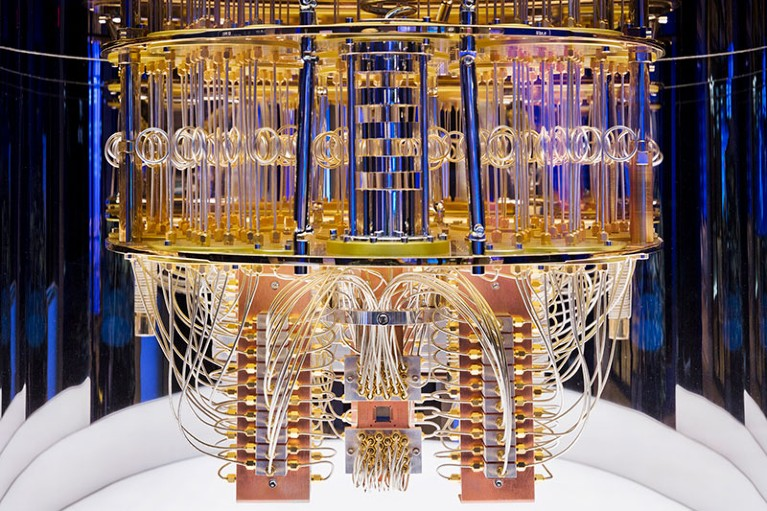
\includegraphics[height=2.3in, width=3.2in, viewport=0 0 767 511,clip]{Figures/Quantum_Computing.jpg}
%                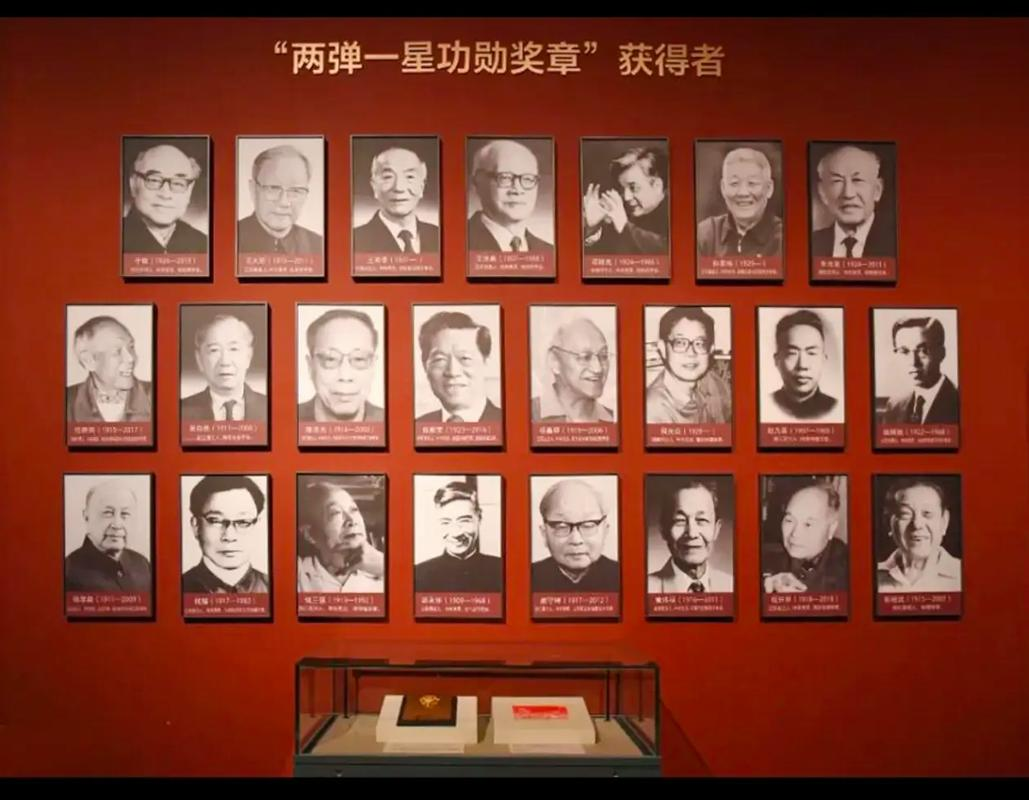
\includegraphics[width=0.95\textwidth]{Figures_History/Collection_23-1.jpeg}
		\caption{\tiny{\textrm{A Schematic illustration of the elements of quantum computing.}}}
		\label{Fig:Quantum_Computing}
            \end{figure}
\end{frame}

\begin{frame}
%	\frametitle{\textrm{EPR佯谬}}
	\frametitle{\textrm{Bell}不等式}
	\begin{itemize}
		\item \textrm{Einstein}与\textrm{Bohr}的辩论
            \begin{figure}
        \centering
                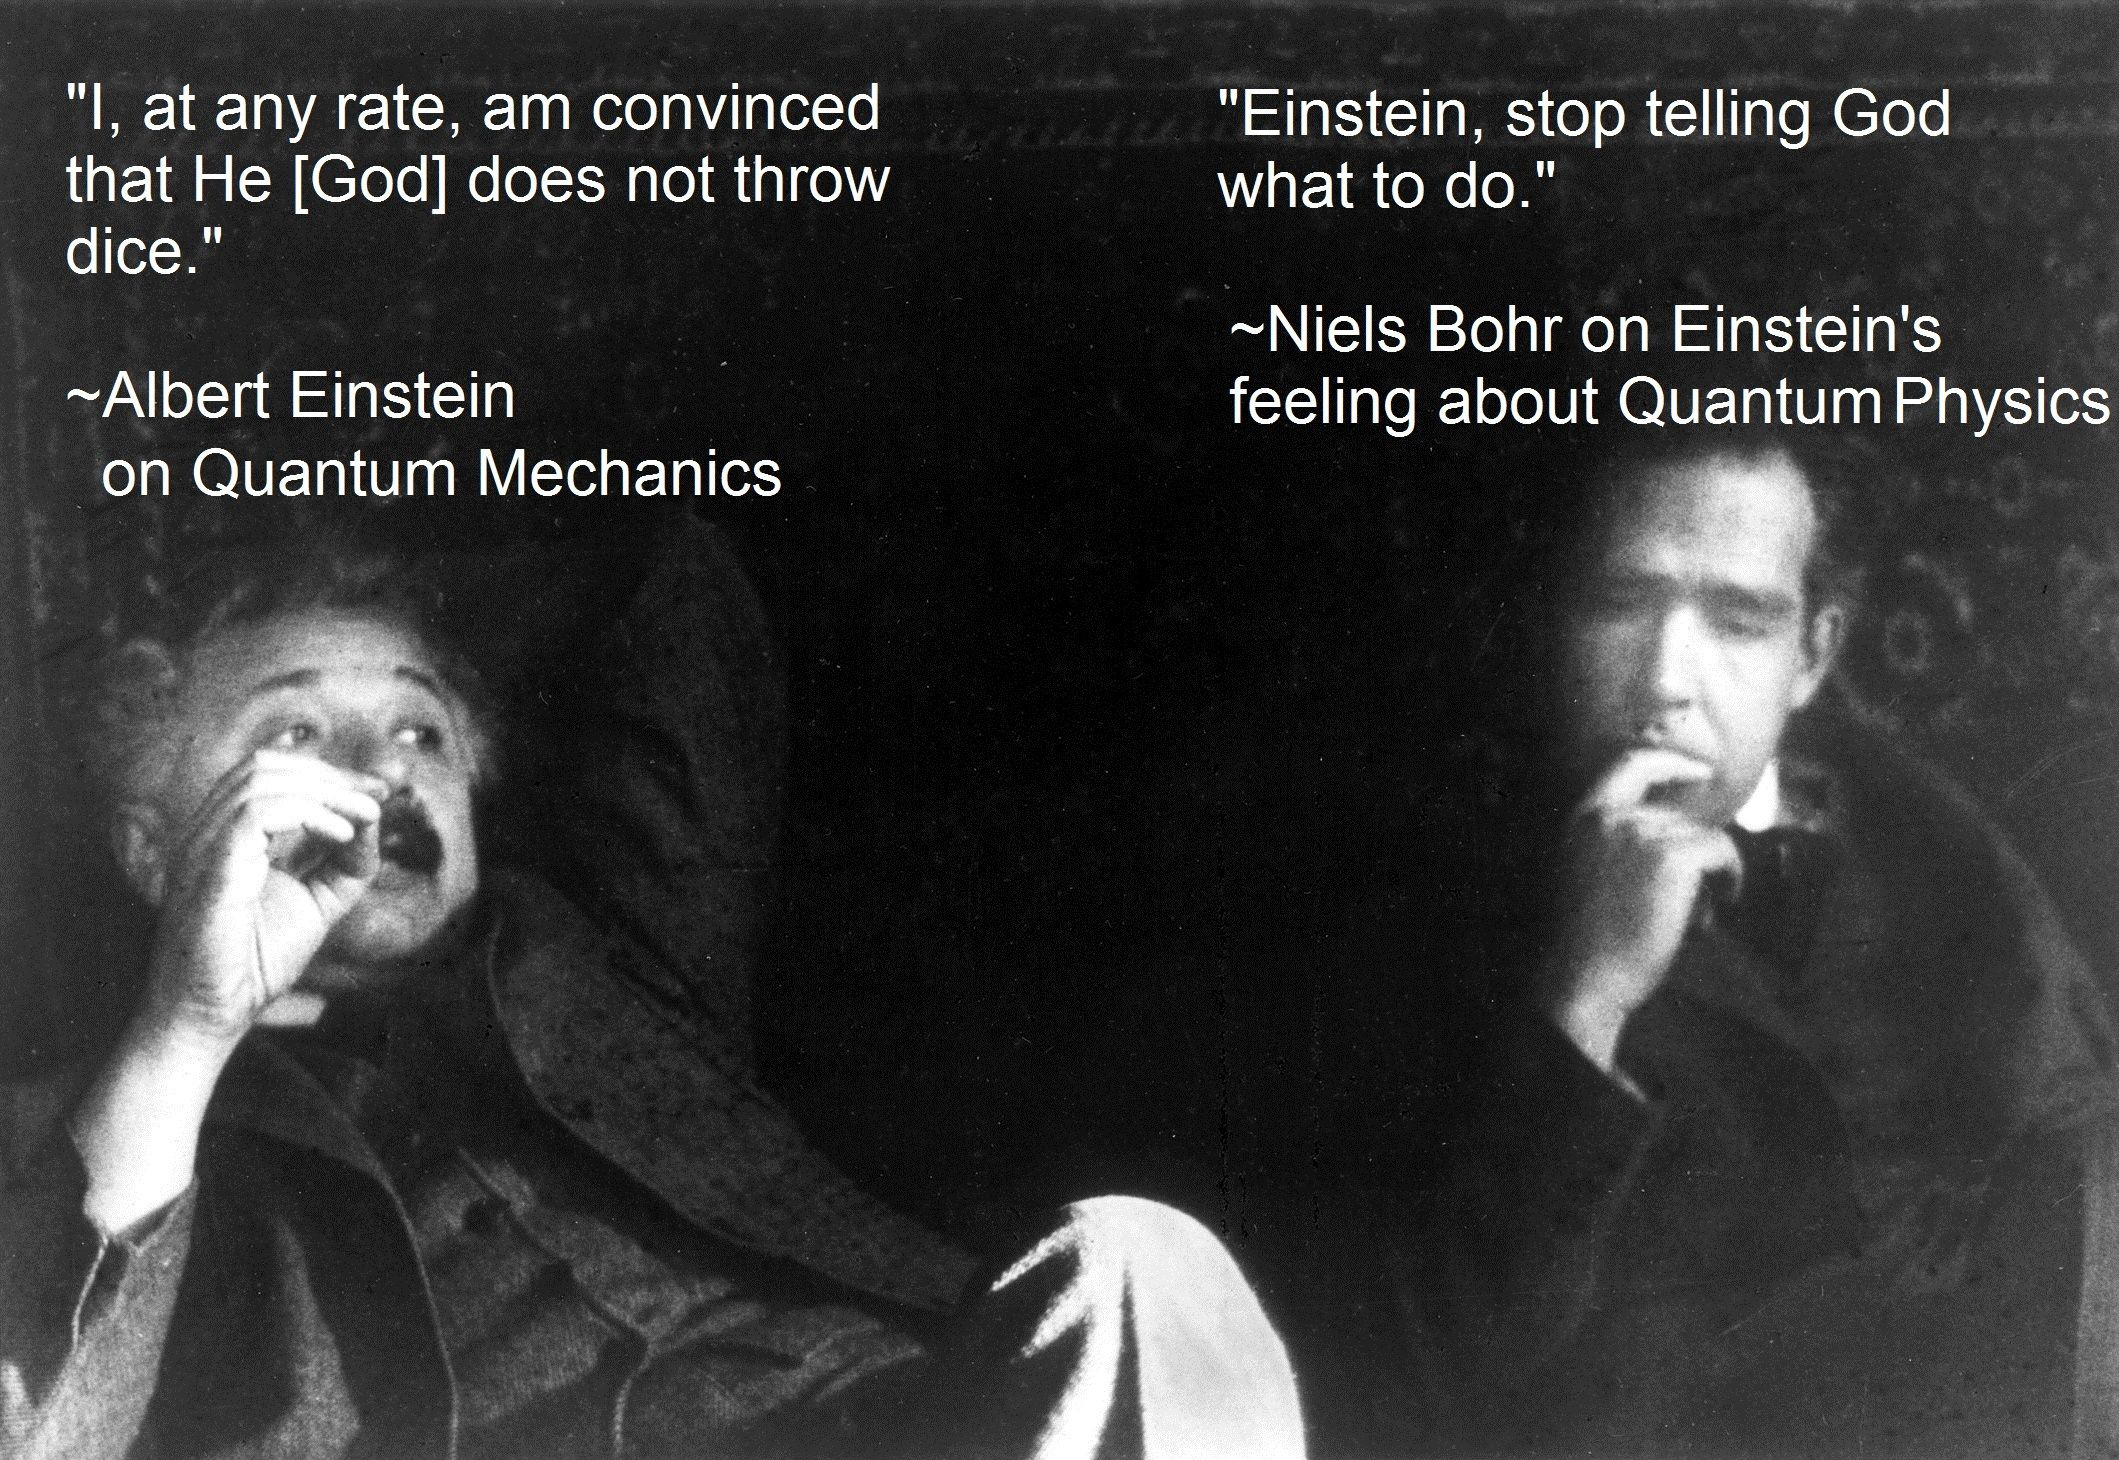
\includegraphics[height=1.4in, width=2.1in, viewport=0 0 2119 1460,clip]{Figures/Einstein-and-Bohr-debate.jpg}
%%		\caption{\tiny{\textrm{Schematic diagram of the entanglement of two qubits.}}}
		\label{Fig:Einstein-Bohr}
            \end{figure}
%    \item \textcolor{red}{\textrm{EPR}佯谬}:
%            \begin{figure}
%	\centering
%                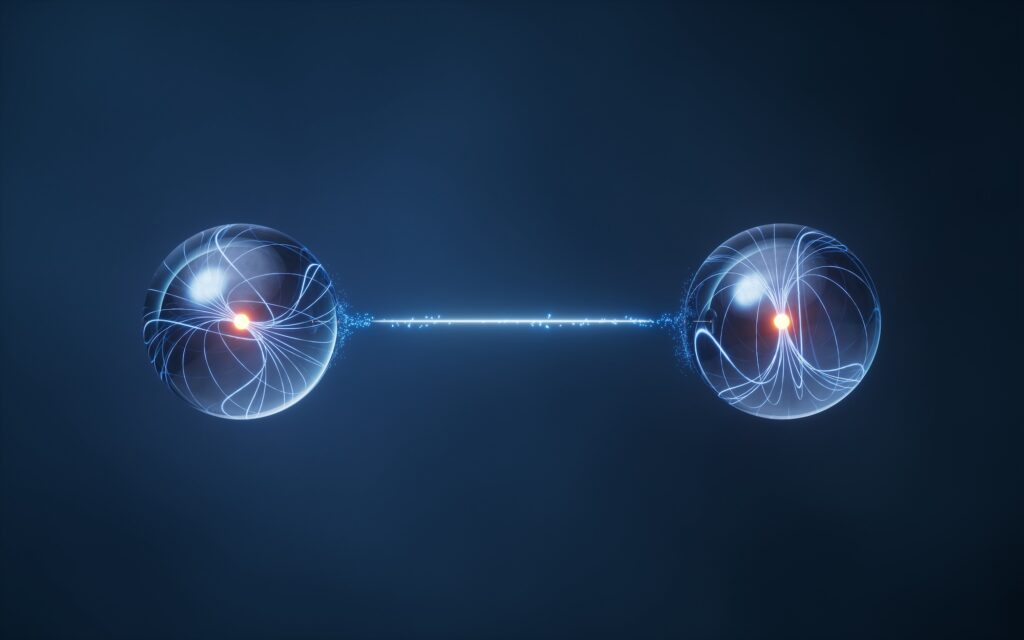
\includegraphics[height=0.4in, width=0.7in, viewport=0 0 250 160,clip]{Figures/Leveraging_principles-of-quantum_mechanics-to-securely-transmit_messages-has-promised-a-revolution-in-encryption_keeping-sensitive-information_secure.jpg}
%%		\caption{\tiny{\textrm{Leveraging principles of quantum mechanics to securely transmit messages has promised a revolution in encryption keeping sensitive information secure.}}}
%		\label{Fig:Leveraging_principles-of-quantum_mechanics-to-securely-transmit_messages-has-promised-a-revolution-in-encryption_keeping-sensitive-information_secure}
%            \end{figure}
%	    {\fontsize{7.5pt}{5.2pt}\selectfont{根据量子力学,假设两个处于纠缠态的粒子(如自旋纠缠的粒子对)被分离到极远距离(如银河系两端),未测量前的粒子处于叠加态(如自旋同时为``$\uparrow$''和``$\downarrow$''的叠加),而测量其中一个粒子会瞬间确定另一个粒子的状态,即使它们相隔达到光年或更远}}
%	\end{itemize}
%	    {\fontsize{7.5pt}{5.2pt}\selectfont{\textrm{Einstein}根据定域实在性主张:~粒子状态在测量前已确定(\textcolor{blue}{存在隐变量}),\underline{\textcolor{purple}{量子力学的不确定性仅源于理论不完备}}\\
%	    \textrm{Bohr}等人基于\textrm{Copenhagen }诠释认为:~\underline{\textcolor{red}{量子态本质是概率性的}},测量导致波函数坍缩,纠缠粒子属于同一系统,无需超距作用}}
%\end{frame}
%
%\begin{frame}
%	\frametitle{隐变量与\textrm{Bell}不等式}
%	\begin{itemize}
%    \item \textrm{Bohm}隐变量理论\\
%	    {\fontsize{8.5pt}{5.2pt}\selectfont{
%		    考虑两个自旋为\textrm{1/2}的粒子\textcolor{blue}{A}和\textcolor{blue}{B}构成的一个体系,在一定时刻后,使\textcolor{blue}{A}和\textcolor{blue}{B}完全分离,不再相互作用:\\
%	    \textcolor{red}{当观察者测得\textcolor{blue}{A}自旋的某一分量后,根据角动量守恒,就能确定地预言\textcolor{blue}{B}在相应\textrm{EPR}佯谬方向上的自旋值}
%		    \begin{enumerate}
%			    \item 微观粒子可以有确定的位置和动量,因此可以用明确的径迹(\textrm{trajectory})描述其运动\\
%				    \textcolor{blue}{但对于粒子位置和速度的测量,依然必须遵守不确定性原理}
%			    \item 粒子接受波函数的引导,并通过与量子势\textrm{(Quantum potential)}的交互作用,表现出非局域的整体性
%			    \item 波函数遵守\textrm{Schr\"odiner}波动方程演化,从不坍缩
%		    \end{enumerate}
%}} 
%隐变量理论可以完全重现与传统统计性量子力学的相同的实验结果
     \item \textrm{Bell}不等式:~{\fontsize{8.5pt}{5.2pt}\selectfont{由\textrm{J.S. Bell}于\textrm{1964}年提出}}
	\begin{displaymath}
		\big|\mathbf{P}_{xy}-\mathbf{P}_{zy}\big|\leqslant 1+\mathbf{P}_{xy}
	\end{displaymath}
	{\fontsize{8.5pt}{5.2pt}\selectfont{\textcolor{magenta}{在定域性和实在性的双重假设下,对于两个分离的粒子同时被测量时,其结果的可能的关联程度给出严格的限制}}}
	\end{itemize}
\end{frame}

\begin{frame}
    \frametitle{量子纠缠原理}
    量子纠缠\textrm{(Quantum entanglement)}是指多个量子比特之间存在一种特殊的关联,使一个量子比特的状态会瞬间影响其他纠缠量子比特的状态,无论它们相距多远
            \begin{figure}
        \centering
                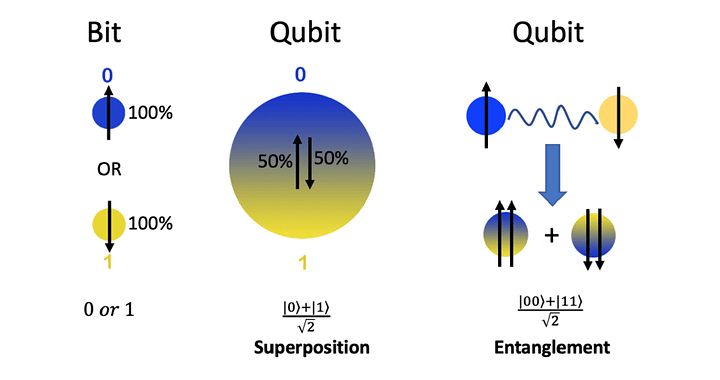
\includegraphics[height=1.5in, width=0.8in, viewport=460 0 645 380,clip]{Figures/Illustration-of-a-bit_and_qubit.png}
                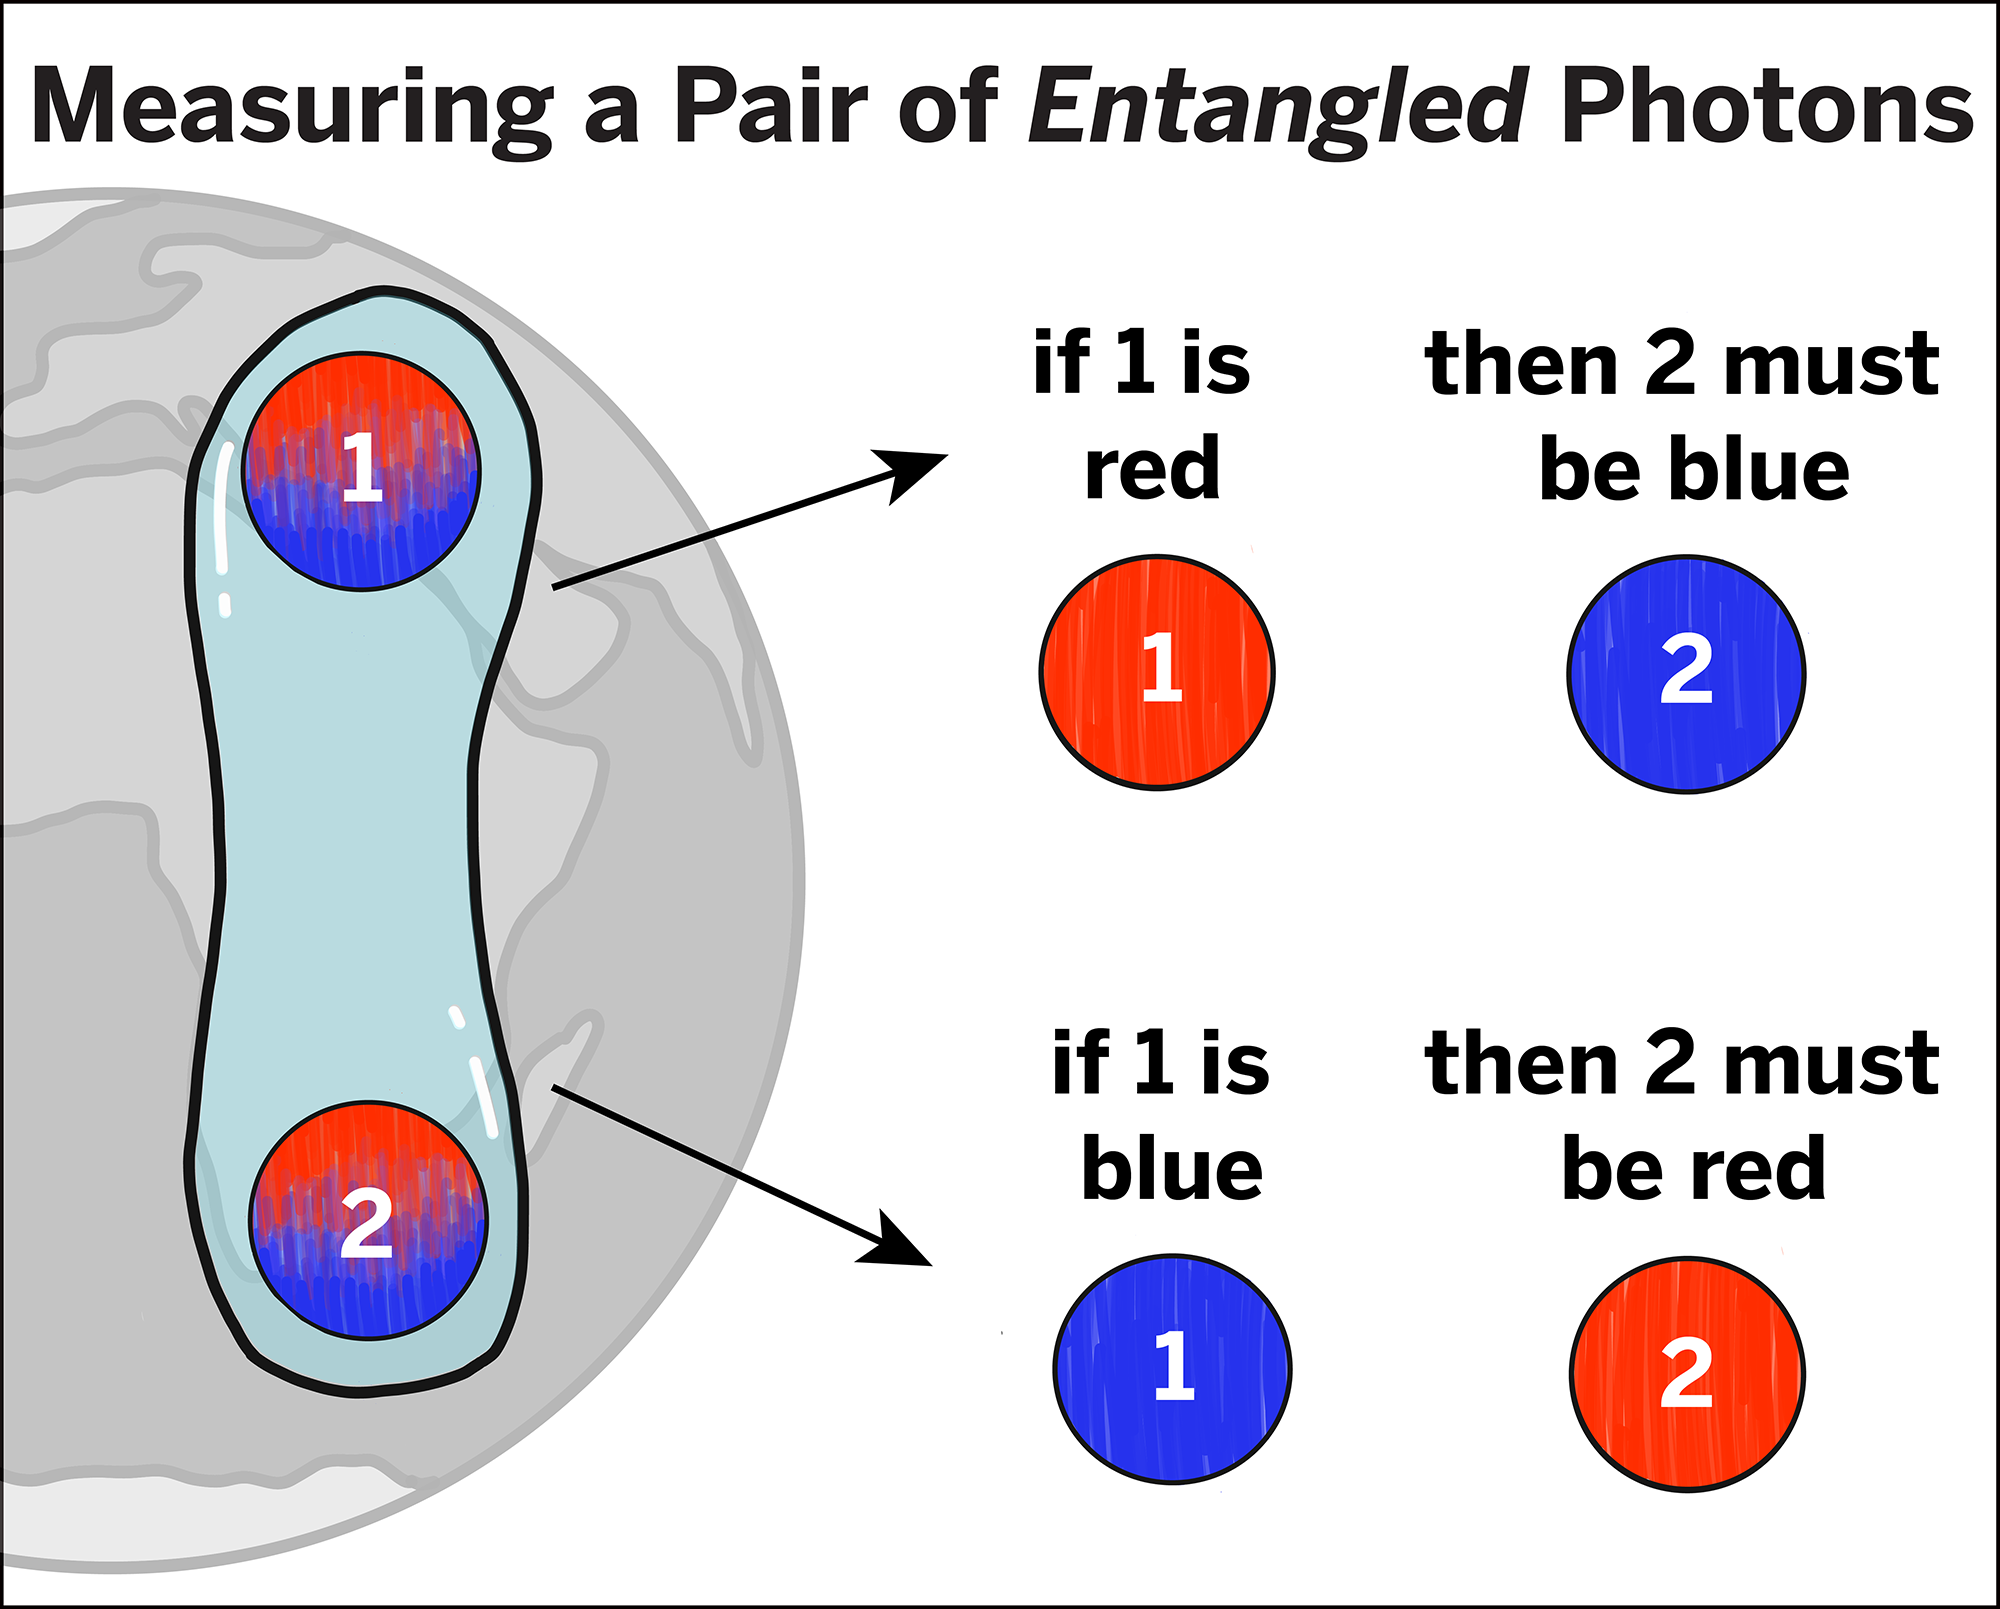
\includegraphics[height=1.5in, width=2.05in, viewport=0 0 980 775,clip]{Figures/Quantum_Entanglement_chart.png}
%                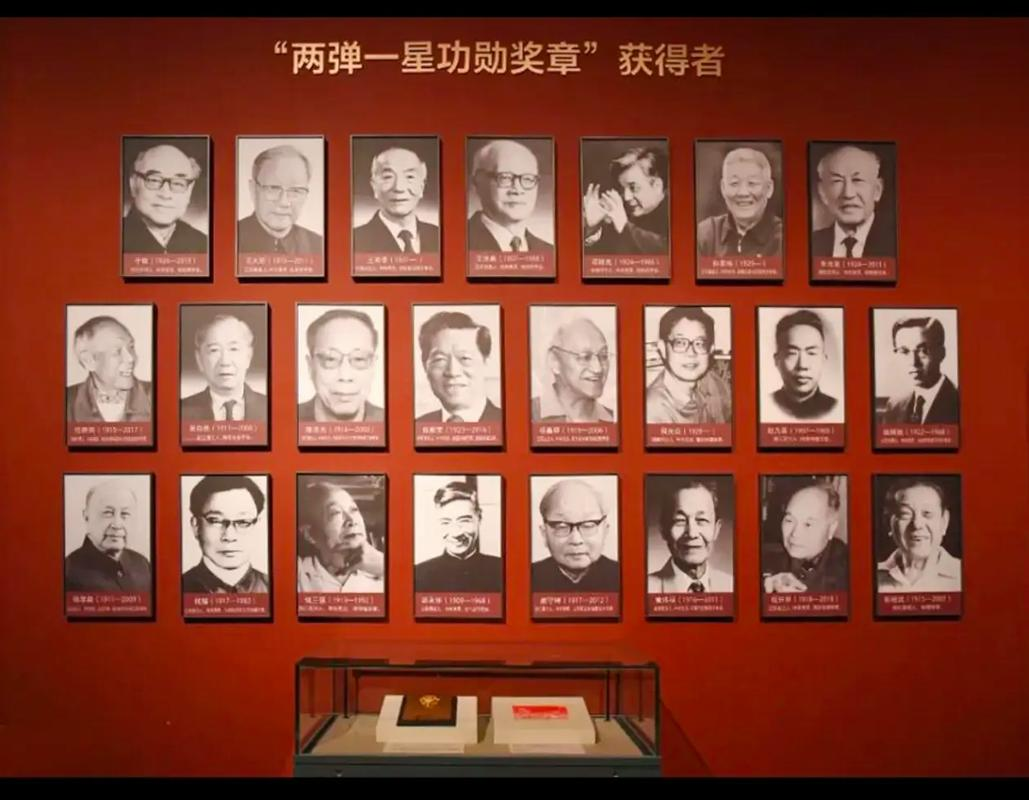
\includegraphics[width=0.95\textwidth]{Figures_History/Collection_23-1.jpeg}
		\caption{\tiny{\textrm{Schematic diagram of the entanglement of two qubits.}}}
		\label{Fig:Illustration-of-a-qubit-entanglement}
            \end{figure}
	    \vskip -10pt
	    {\fontsize{7.5pt}{5.2pt}\selectfont{利用量子纠缠可以实现高效的信息传输和处理,是量子通信和量子计算的重要资源}}
\end{frame}

\begin{frame}
    \frametitle{量子门操作}
    与经典计算机中的逻辑门\textrm{(如与门/And、或门/Or等)}类似,量子计算机通过量子门对量子比特进行操作\\
{\fontsize{7.5pt}{5.2pt}\selectfont{常见的量子门有 \textrm{Pauli} 门\textrm{(X、Y、Z 门)}、\textrm{Hadamard} 门、\textrm{CNOT} 门等,这些门操作可以改变量子比特的状态和相位}}
    \begin{figure}
        \centering
        % 这里可以插入量子门操作的示意图片
                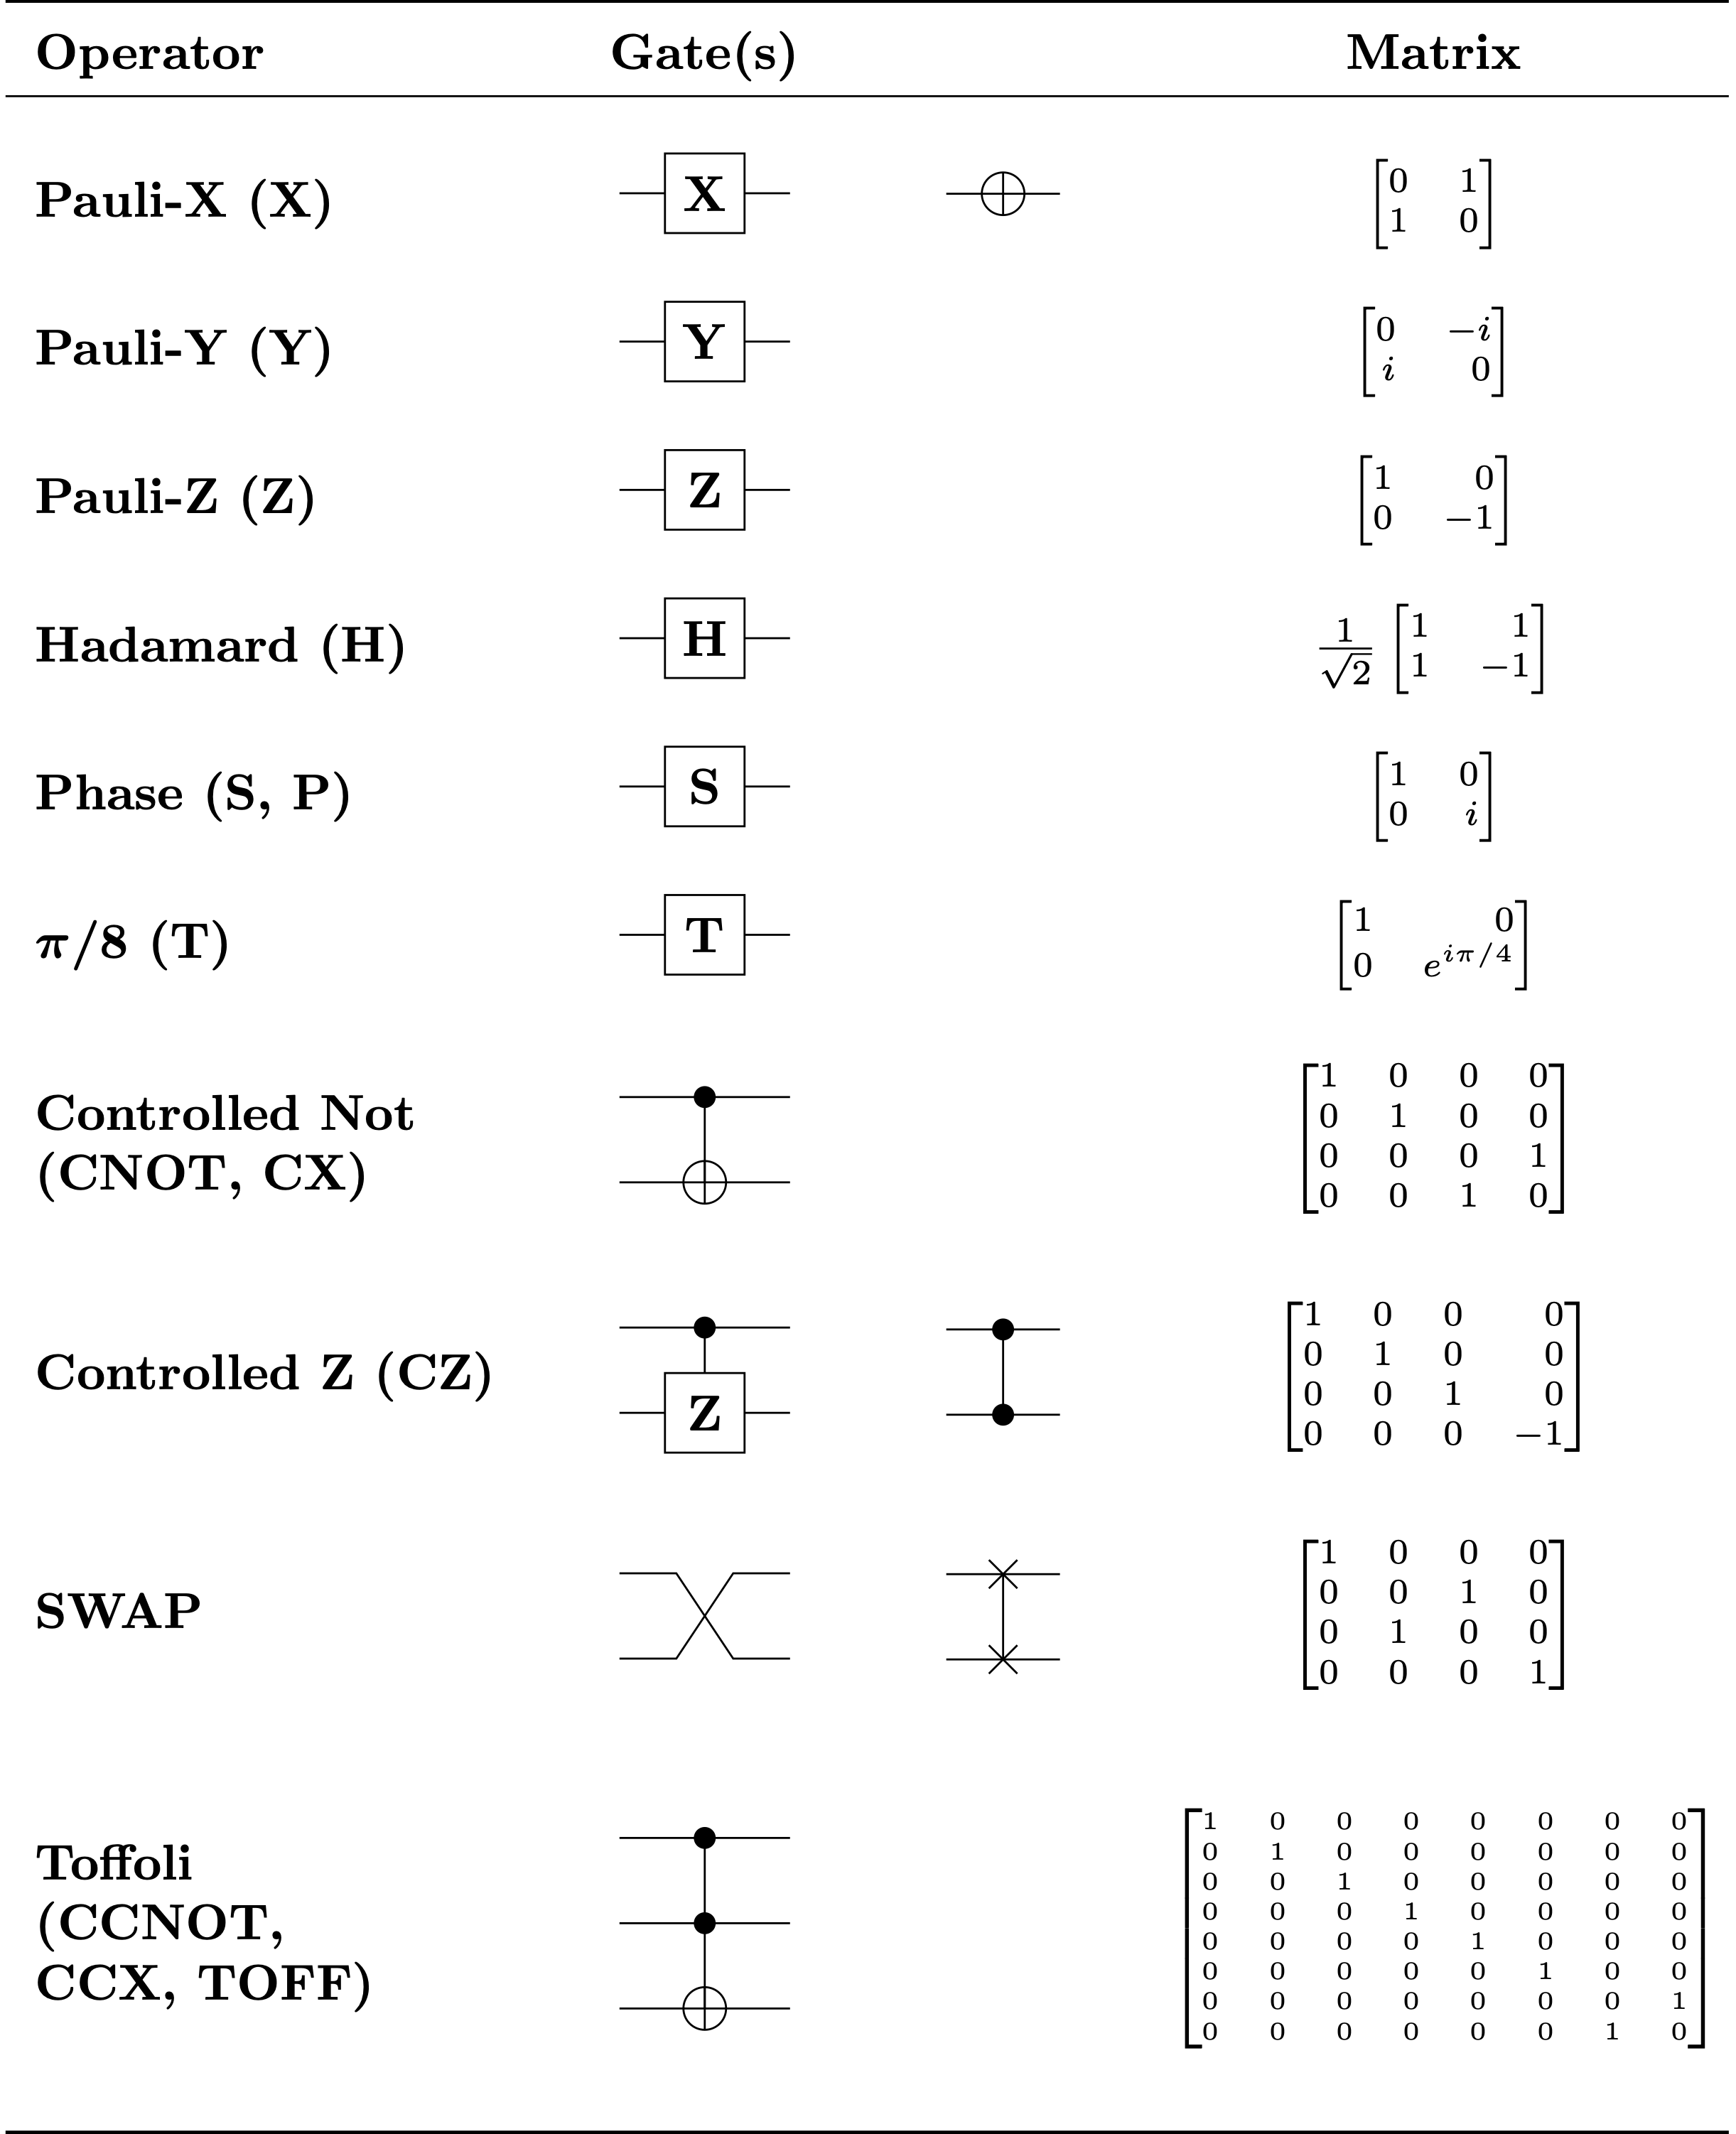
\includegraphics[height=1.7in, width=1.5in, viewport=0 0 390 430,clip]{Figures/Quantum_Logic_Gates.png}
		\caption{\tiny{\textrm{Common quantum logic gates by name (including abbreviation), circuit form(s) and the corresponding unitary matrices.}}}
		\label{Fig:Quantum_Logic_Gates}
    \end{figure}
\end{frame}

% 生成量子态技术部分
\section{量子态生成技术}
\begin{frame}
    \frametitle{激光冷却与俘获技术}
%    \begin{itemize}
    \textcolor{blue}{原理}:~利用激光与原子的相互作用,通过原子随机运动和辐射光子来冷却和俘获原子,将原子的运动速度降低到极低水平,从而使其处于特定的量子态
%    \end{itemize}
    \begin{figure}
        \centering
                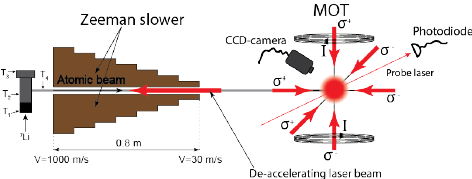
\includegraphics[height=1.5in, width=3.9in, viewport=0 0 472 179,clip]{Figures/Optical-scheme-of-laser-cooling-and-trapping-for-lithium-atoms.png}
        % 这里可以插入激光冷却与囚禁技术的示意图片
		\caption{\tiny{\textrm{Optical scheme of laser cooling and trapping for lithium atoms.}}}
		\label{Fig:Optical-scheme-of-laser-cooling-and-trapping-for-lithium-atoms}
    \end{figure}
	    \vskip -10pt
    {\fontsize{7.5pt}{5.2pt}\selectfont{\textcolor{blue}{应用}:~在离子阱量子计算机中,激光冷却与俘获技术可用于制备和控制离子的量子态,为量子计算提供稳定的\textrm{qubit}}}
\end{frame}

\begin{frame}
    \frametitle{激光冷却与俘获:~\textrm{Doppler}冷却}
	    利用\textrm{Doppler}效应冷却原子
    \begin{figure}
        \centering
                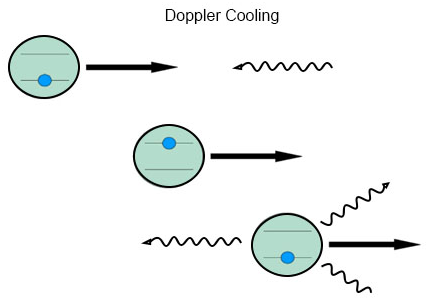
\includegraphics[height=1.5in, width=2.2in, viewport=0 0 429 307,clip]{Figures/Atom-MOT-and-laser-cooling_Doppler_cooling.png}
        % 这里可以插入激光冷却与囚禁技术的示意图片
		\caption{\tiny{\textrm{Schematic diagram of Doppler cooling.}}}
		\label{Fig:Atom-MOT-and-laser-cooling_Doppler_cooling}
    \end{figure}
	    {\fontsize{8.5pt}{5.2pt}\selectfont{将激光的频率调到略低于原子的跃迁频率:~
		    \begin{itemize}
			    \item 当激光束与原子相向运动,其频率略微蓝移,因此原子将吸收光子
		    \item 当原子与激光束背向运动,将感受到红移后的激光频率,而释放光子
		    \end{itemize}
	    最终使得原子损失动能,达到冷却的目的}}
\end{frame}

\begin{frame}
	\frametitle{激光冷却与俘获:~\textrm{Zeeman}减速}
	\textrm{Zeeman}减速利用磁场梯度来俘获原子
    \begin{figure}
        \centering
                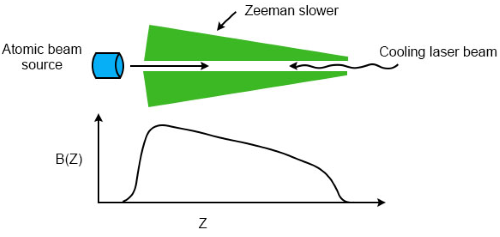
\includegraphics[height=1.5in, width=3.1in, viewport=0 0 500 237,clip]{Figures/Atom-MOT-and-laser-cooling_Zeeman_slower.png}
        % 这里可以插入激光冷却与囚禁技术的示意图片
		\caption{\tiny{\textrm{Schematic diagram of Zeeman slower.}}}
		\label{Fig:Atom-MOT-and-laser-cooling_Zeeman_slower}
    \end{figure}
	    \vskip -10pt
	    \textcolor{magenta}{\textrm{Zeeman}减速是对\textrm{Doppler}冷却的延伸:}\\
	{\fontsize{8.5pt}{5.2pt}\selectfont{伴随着原子沿激光传播方向速度的减速,将被\textrm{Doppler}效应更有效地冷却}}
\end{frame}

\begin{frame}
	\frametitle{激光冷却与俘获:~磁-光俘获}
	磁-光俘获\textrm{(Magneto-Optical Traps, MOTs)}:~将磁场和激光束相结合,用以捕获超冷原子
    \begin{figure}
        \centering
                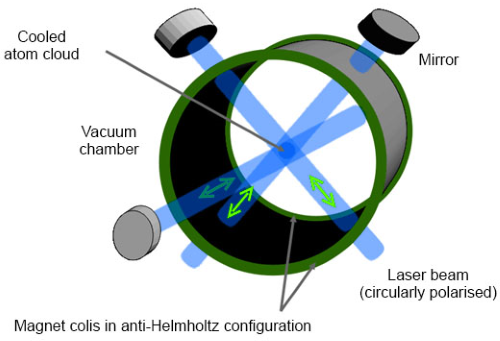
\includegraphics[height=1.5in, width=2.2in, viewport=0 0 500 341,clip]{Figures/Atom-MOT-and-laser-cooling_MOTs.png}
        % 这里可以插入激光冷却与囚禁技术的示意图片
		\caption{\tiny{\textrm{Schematic diagram of Magneto-Optical Traps.}}}
		\label{Fig:Atom-MOT-and-laser-cooling_MOTs}
    \end{figure}
	    \vskip -10pt
    {\fontsize{7.5pt}{5.2pt}\selectfont{由多束对向激光束构成稳定的区域,并利用磁场将原子约束在该区域:\\
    原子在该区域内运动时,将感受到指向激光束束心的回复力。由此将形成冷原子凝聚云,并可以长期保持}}
\end{frame}

\begin{frame}
	\frametitle{\textrm{Josephson-junction}技术}
%    \begin{itemize}
		    \textrm{Josephson-junction}是由两个超导体之间夹一层薄绝缘层构成的结构\\
		    {\fontsize{7.5pt}{5.2pt}\selectfont{通过控制\textrm{Josephson-junction}中的电流和电压,可以实现超导\textrm{qubit}的制备和操作,从而生成特定的量子态}}
%    \end{itemize}
    \begin{figure}
        \centering
                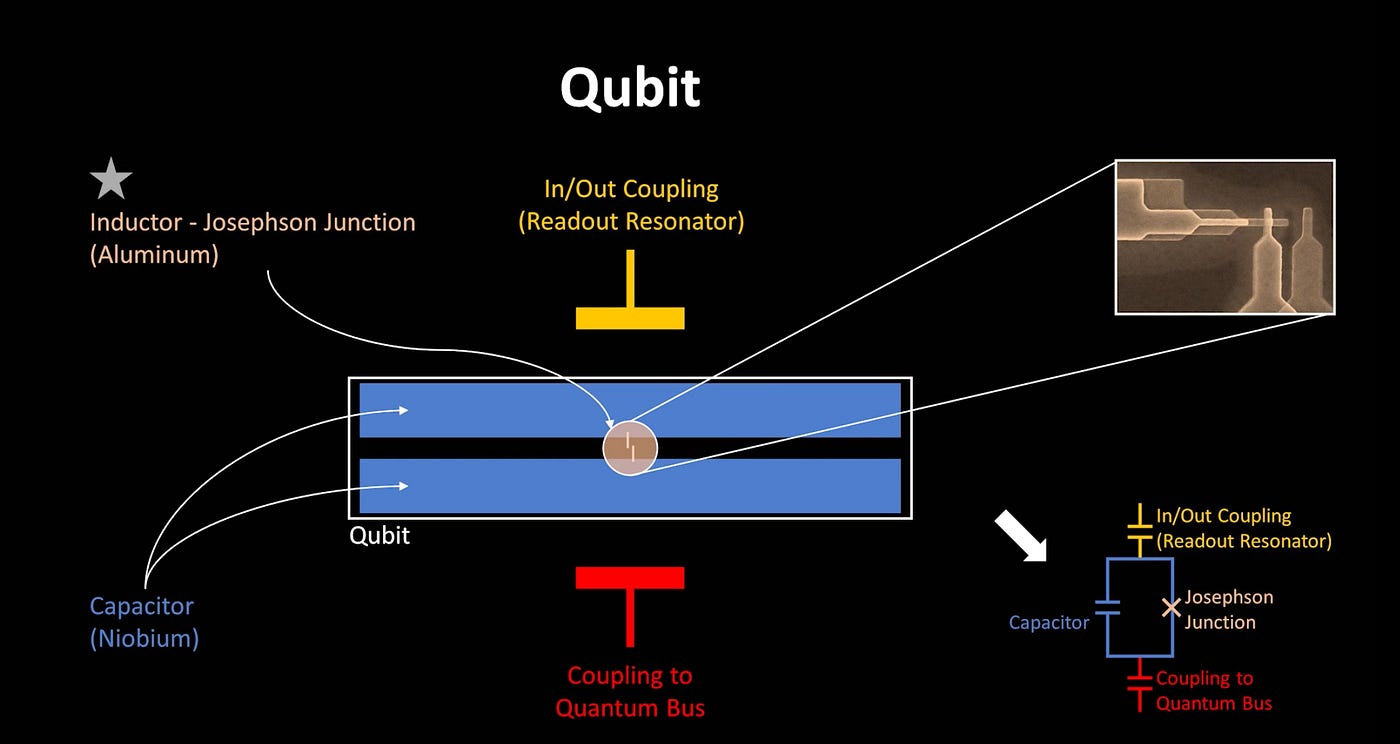
\includegraphics[height=1.5in, width=2.6in, viewport=0 0 1400 744,clip]{Figures/Schematic-Josephson_junction-for-qubit.jpg}
        % 这里可以插入激光冷却与囚禁技术的示意图片
		\caption{\tiny{\textrm{Schematic diagram of Josephson-junction for qubit.}}}
		\label{Fig:Josephson-junction}
    \end{figure}
	    \vskip -10pt
    {\fontsize{7.5pt}{5.2pt}\selectfont{%在超导量子计算中,
	    \textrm{Josephson-junction}%是构建量子比特的关键元件,
    广泛应用于量子芯片的制造中}}
\end{frame}

\begin{frame}
    \frametitle{量子点}
%    \begin{itemize}
        量子点是一种纳米尺度的半导体结构,电子能级具有离散性\\
	{\fontsize{8.5pt}{5.2pt}\selectfont{通过控制量子点中的电子数量和能级结构,可以实现对量子态的精确调控}}
%    \end{itemize}
    \begin{figure}
        \centering
                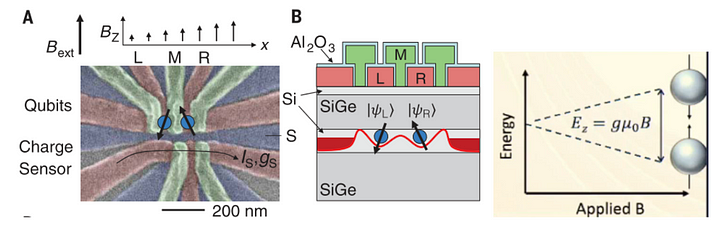
\includegraphics[height=1.2in, width=4.0in, viewport=0 0 720 237,clip]{Figures/Si_SiGe-heterostructure_QD-spin_up-and-spin_down-electrons-have-a-different-energy.png}
        % 这里可以插入激光冷却与囚禁技术的示意图片
		\caption{\tiny{\textrm{This is a Si/SiGe heterostructure; here, the QD is designed such that spin-up and spin-down electrons have a different energy, allowing to address the spins separately.}}}
		\label{Fig:Si_SiGe-heterostructure_QD-spin_up-and-spin_down-electrons-have-a-different-energy}
%                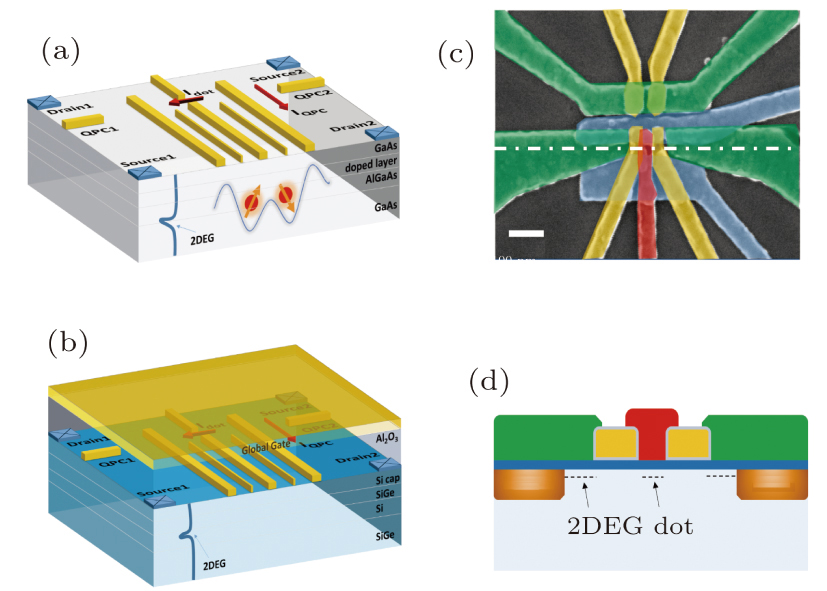
\includegraphics[height=1.5in, width=2.6in, viewport=0 0 827 591,clip]{Figures/Device_structure-of-the-semiconductor_quantum_dot-with-doped-AlGaAs_GaAs-heterostructure-and-undoped_Si_SiGe herterostructure.jpg}
%		\caption{\tiny{\textrm{Device structure of the semiconductor quantum dot. Panels (a) and (b) are schematics of a double quantum dot fabricated using doped AlGaAs/GaAs heterostructure and undoped Si/SiGe herterostructure, respectively. is the current from source to drain through the dot, while is the current from source to drain through the QPC channel. The location of 2DEG and the electrons with spin directions in the double quantum dot are also shown. (c) Scanning electron micrograph (SEM) of a CMOS quantum dot with a SET as a charge sensor, where a white dash dotted line shows position of the cross section (d). Confinement gates (blue), lead gates (green), barrier gates (orange), and plunger gates (red) are shown. (d) Cross section of a CMOS quantum dot, dotted lines denote where 2DEG and a quantum dot form..}}}
%		\label{Fig:Device_structure-of-the-semiconductor_quantum_dot-with-doped-AlGaAs_GaAs-heterostructure-and-undoped_Si_SiGe herterostructure}
    \end{figure}
       	    \vskip -10pt
	    {\fontsize{9.5pt}{5.2pt}\selectfont{在半导体量子计算中,量子点可作为量子比特的载体,用于生成和处理量子信息}}
\end{frame}

%% 量子态的保持部分
%\section{量子态的保持}
%\begin{frame}
%    \frametitle{量子态保持的重要性}
%    \begin{itemize}
%        \item 在量子计算、量子通信和量子加密中,准确的量子态是实现各项功能的基础。
%        \item 若量子态不能有效保持,将导致计算结果出错、通信信息丢失以及加密安全性降低等问题。
%    \end{itemize}
%\end{frame}
%
%\begin{frame}
%    \frametitle{低温环境控制}
%    \begin{itemize}
%        \item 原理:热噪声是导致量子态退相干的重要因素之一。将量子系统置于极低温度环境下,可减少热噪声对量子态的干扰。
%	\item 例如,超导量子比特通常需要在接近绝对零度\textrm{(约 -273.15$^{\circ}\mathrm{C}$)}的极低温环境中工作,以保持其量子态的稳定性。
%    \end{itemize}
%    \begin{figure}
%        \centering
%        % 这里可以插入低温环境控制设备的图片
%        \caption{低温环境控制设备}
%    \end{figure}
%\end{frame}
%
%\begin{frame}
%    \frametitle{电磁屏蔽}
%    \begin{itemize}
%        \item 原理:外界的电磁场会与量子系统相互作用,破坏量子态的相干性。采用电磁屏蔽措施,可阻挡外界电磁场的干扰。
%        \item 常见的电磁屏蔽材料有金属屏蔽罩等,将量子系统封装在屏蔽罩内,可有效减少电磁干扰。
%    \end{itemize}
%    \begin{figure}
%        \centering
%        % 这里可以插入电磁屏蔽的示意图片
%        \caption{电磁屏蔽示意图}
%    \end{figure}
%\end{frame}
%
\begin{frame}
    \frametitle{量子纠错编码}
        量子纠错码是一种通过引入冗余信息来检测和纠正量子态错误的技术\\
	{\fontsize{7.5pt}{5.2pt}\selectfont{当量子态受到干扰发生错误时,量子纠错码可以识别并恢复正确的量子态}}
    \begin{figure}
        \centering
                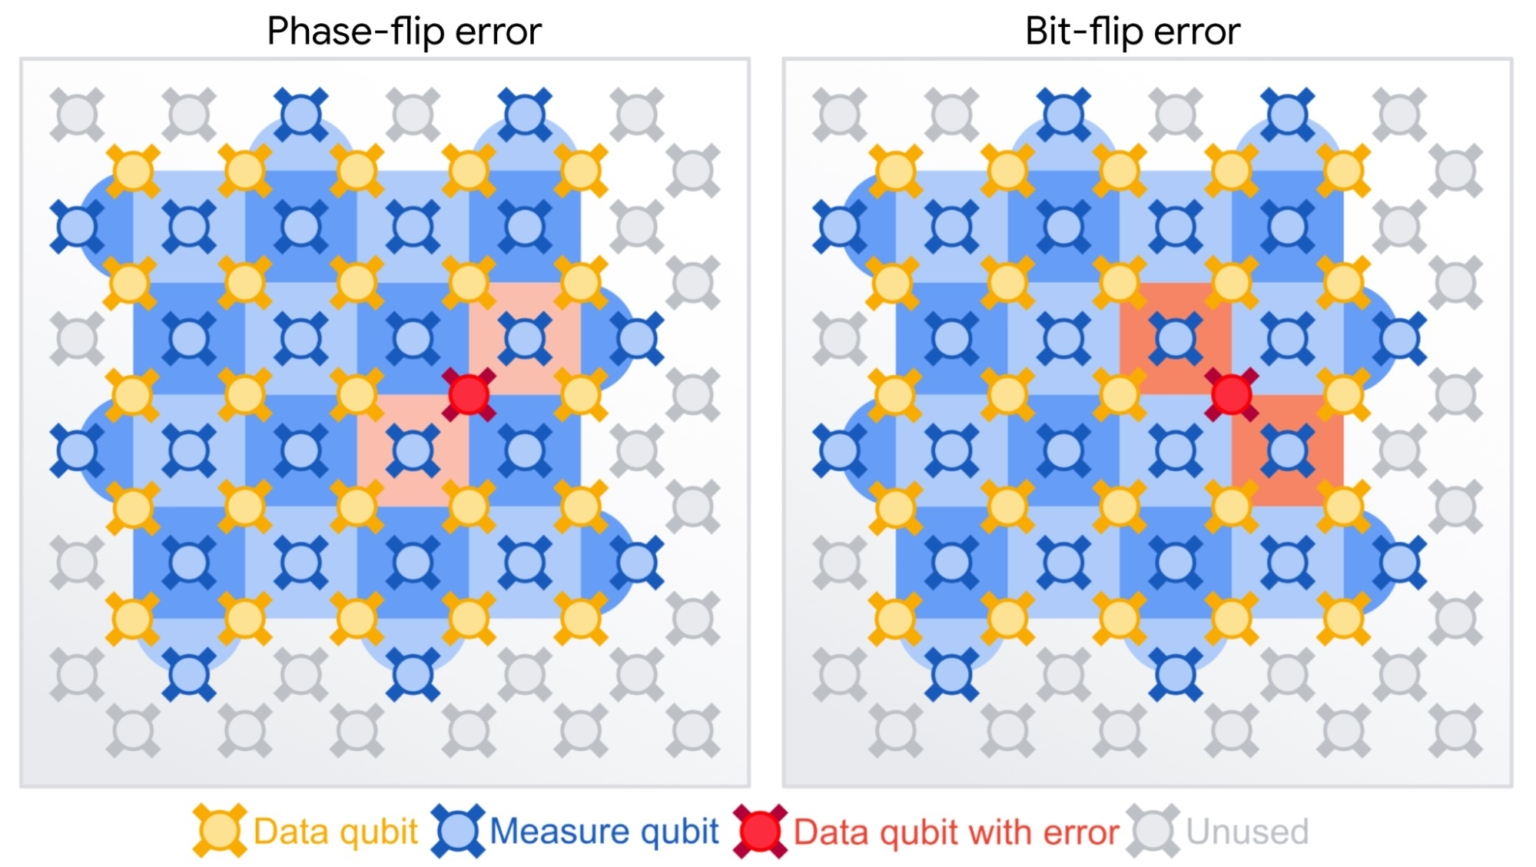
\includegraphics[height=1.2in, width=2.3in, viewport=0 0 1210 650,clip]{Figures/Quantum_Error-correction-diagram.jpg}
		\caption{\tiny{\textrm{Surface code: illustration of how error correction works for bit and phase flips. The measure qubits on light blue backgrounds check for phase flip errors while the measure qubits on dark blue backgrounds check for bit flip errors. In this example the measure qubits on reddish backgrounds are registering the errors.}}}
		\label{Fig:Quantum_Error-correction-diagram}
    \end{figure}
       	    \vskip -10pt
	    {\fontsize{7.5pt}{5.2pt}\selectfont{表面编码是一种常用的量子纠错码,在量子计算中可有效提高量子态的保持时间和计算的可靠性}}
\end{frame}

% 量子通信部分
\section{量子通信与加密}
\begin{frame}
    \frametitle{量子通信}
    \textcolor{red}{量子通信}:~利用量子力学原理,依赖量子相干态进行信息传输
    {\fontsize{7.5pt}{5.2pt}\selectfont{主要方式包括}}:
    \begin{itemize}
	\item 量子密钥分发\textrm{(Quantum Key Distribution,~QKD)}
	\item 量子隐形传态\textrm{(Quantum Teleportation,~QT)}
    \end{itemize}
    \begin{figure}
        \centering
                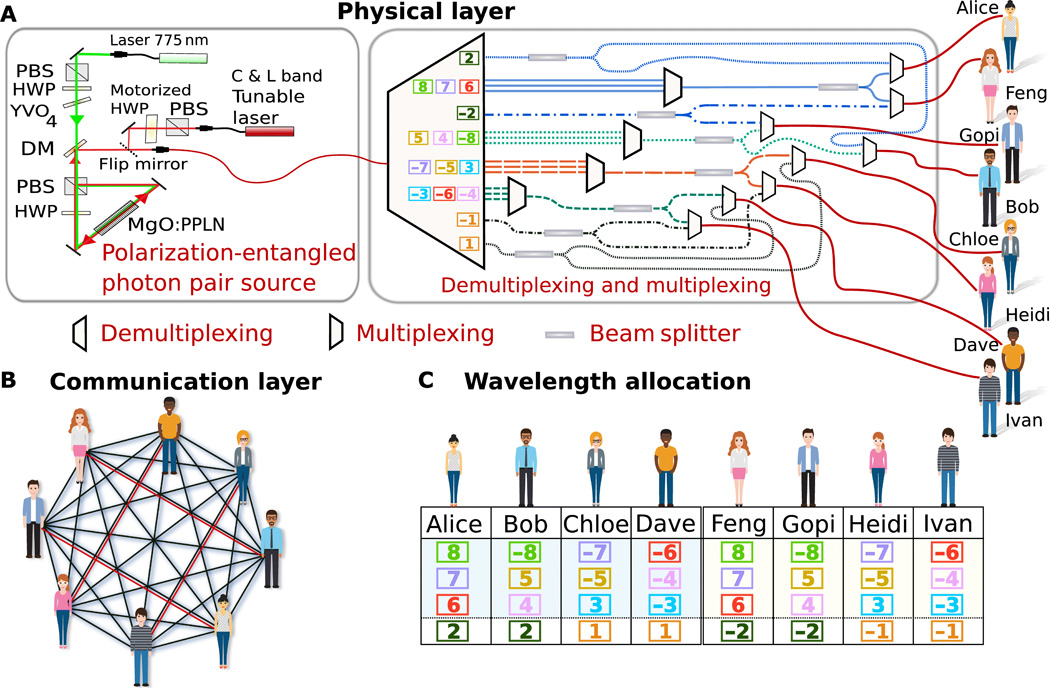
\includegraphics[height=1.7in, width=3.0in, viewport=0 0 1050 688,clip]{Figures/Quantum_Communication.jpeg}
		\caption{\tiny{\textrm{The overall network architecture showing the physical layer, communication layer, and the way wavelength channels are distributed.}}}%The network consists of two layers. (A) The physical layer contains the source of entanglement (blue) and the multiplexing unit (MU; gray). These form the QNSP. Our topology uses just one deployed fiber (red) per user to interconnect all eight individual users. (B) The communication layer forms a fully connected graph without trusted nodes for entanglement distribution, key exchange, and secure communication (classical communication channels between users are not shown). Each line represents a link—the sharing of a bipartite entangled state. Higher-bandwidth links share a second entangled state shown as a red line. (C) Wavelength allocation: Every user of the eight-node network receives four wavelength channels denoted by a number (which corresponds to their ITU 100-GHz DWDM grid channel number minus 34). That is, ITU channel 34 (or 0 in the figure’s naming convention) corresponds to the channel approximately centered at the down-conversion degeneracy wavelength. Thus, a pair of matching colors or numbers with equal absolute values and opposite sign denote wavelengths corresponding to an entangled photon pair. The regions shaded in blue and yellow are identical subnets and represent the multiplexing using BSs. The last row below the dotted line shows the additional wavelength channel needed to fully interconnect the two subnets. Certain user pairs are connected by two entangled photon pairs (such as Alice and Gopi via {8, −8} and {2, −2}) and consequently enjoy an increased key rate.
		\label{Fig:Quantum_Communication}
    \end{figure}
\end{frame}

\begin{frame}
	\frametitle{量子密钥分发\textrm{(QKD)}}
    \begin{itemize}
        \item 基于量子力学的观测塌缩特性和测不准原理
        \item 可以实现无条件安全的密钥分发,量子相干态的特性保证了密钥的安全性
    \end{itemize}
    \begin{figure}
        \centering
                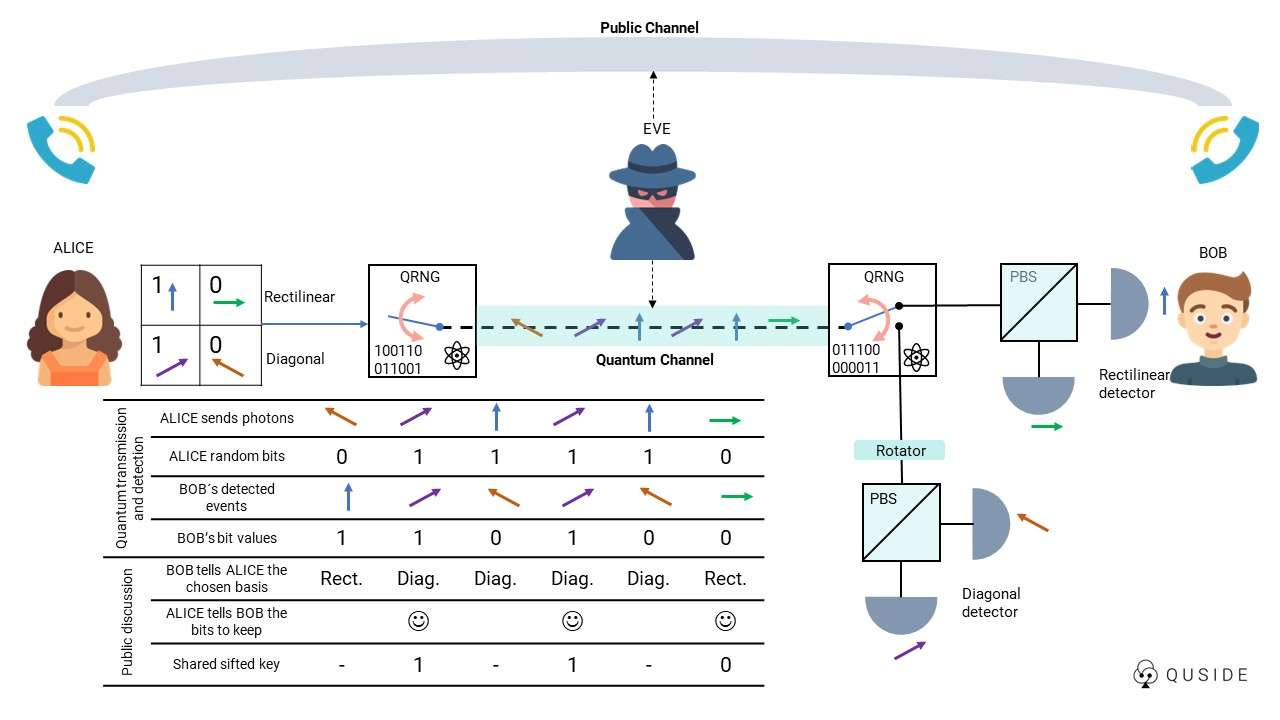
\includegraphics[height=1.5in, width=3.0in, viewport=0 0 1280 720,clip]{Figures/Quantum_Communication-QKD_infografia.jpeg}
		\caption{\tiny{\textrm{Basic principle diagram of using the BB84 protocol in the QKD link.}}}
		\label{Fig:Basic-principle_diagram-of-using-the-BB84_protocol-in-the-QKD-link}
    \end{figure}
\vskip -10pt
{\fontsize{7.5pt}{5.2pt}\selectfont{
    \begin{alertblock}{安全性保障}
        任何对量子态的测量都会改变其状态,从而被通信双方察觉
\end{alertblock}}}
\end{frame}

% 量子隐形传态部分
%\subsection{量子隐形传态}
\begin{frame}
	\frametitle{量子隐形传态\textrm{(QT)}}
        量子隐形传态:~利用量子纠缠实现量子态信息传输的技术\\
	\textcolor{red}{并非是将实体物质进行传输,而是传输量子态所携带的信息}
	\vskip 2pt
    量子隐形传态原理
    \begin{itemize}
	    \item \textcolor{blue}{准备}:~首先制备一对处于纠缠态的量子比特(如光子对)\\
		    {\fontsize{7.5pt}{5.2pt}\selectfont{将其中一个光子发送给发送方\textrm{(Alice)},另一个发送给接收方\textrm{(Bob)}}}
	    \item \textcolor{blue}{编码}:~\textrm{Alice} 拥有一个待传输的量子比特 \( |\psi\rangle \),她对这个量子比特和手中的纠缠光子进行联合测量\\
		    {\fontsize{7.5pt}{5.2pt}\selectfont{\textcolor{magenta}{该次测量会使这两个量子比特的状态发生坍缩,同时由于纠缠关系,\textrm{Bob}手中的光子状态也会相应改变}}}
	    \item \textcolor{blue}{传输}:~\textrm{Alice} 通过经典通信渠道(如光纤、无线电等)将她的测量结果发送给 \textrm{Bob}
	    \item \textcolor{blue}{解码}:~\textrm{Bob}根据接收到的经典信息,对自己手中的光子进行相应的幺正变换操作\\
		    {\fontsize{7.5pt}{5.2pt}\selectfont{使该光子的状态变为 \( |\psi\rangle \),实现了量子态的传输}}
    \end{itemize}
\end{frame}

\begin{frame}
    \frametitle{量子隐形传态的应用}
    \begin{figure}
        \centering
                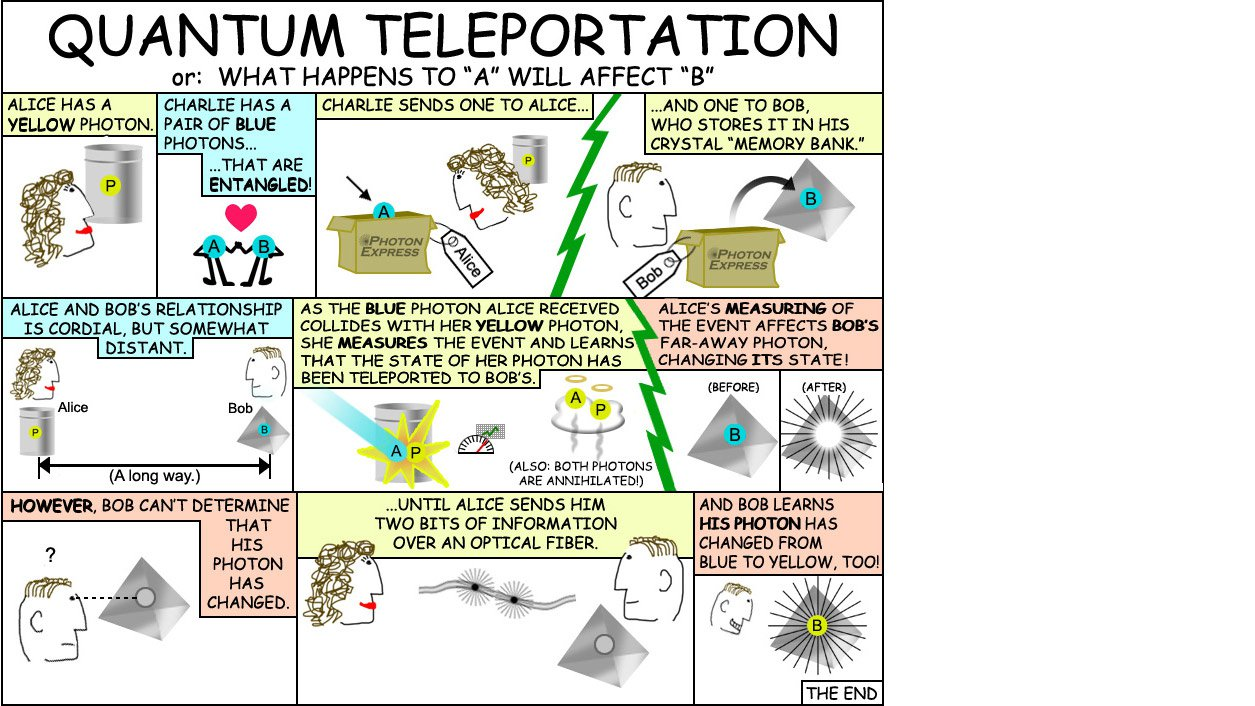
\includegraphics[height=1.2in, width=2.0in, viewport=0 0 900 710,clip]{Figures/Quantum_Teleportation.jpg}
		\caption{\tiny{\textrm{A cartoon-demonstration explains the Quantum Teleportation.}}}
		\label{Fig:Quantum_Teleportation}
    \end{figure}
    \vskip -10pt
    \begin{itemize}
        \item 量子通信网络:~%作为量子通信网络的关键技术,
		实现远程节点之间的量子态传输\\
		{\fontsize{7.5pt}{5.2pt}\selectfont{为构建大规模、长距离的量子通信网络奠定基础}}
        \item 量子计算:~在分布式量子计算中,用于在不同计算单元之间传输量子信息\\
		{\fontsize{7.5pt}{5.2pt}\selectfont{提高计算效率和协同性}}
        \item 量子加密:~保障敏感信息的安全传输\\
		{\fontsize{7.5pt}{5.2pt}\selectfont{结合量子隐形传态和量子密钥分发技术,可进一步增强信息传输的安全性}}
    \end{itemize}
\end{frame}

% 直接量子通信部分
%\subsection{直接量子通信}
\begin{frame}
    \frametitle{量子直接通信}
%    \begin{itemize}
	    量子直接通信\textrm{(Quantum Direct Communication,~QDC)}:\\
		    {\fontsize{7.5pt}{5.2pt}\selectfont{由清华大学龙桂鲁团队原创提出的一种不依赖于传统密钥分发的量子通信方式,能直接在通信双方之间传输信息}}
%    \end{itemize}
    \begin{figure}
        \centering
                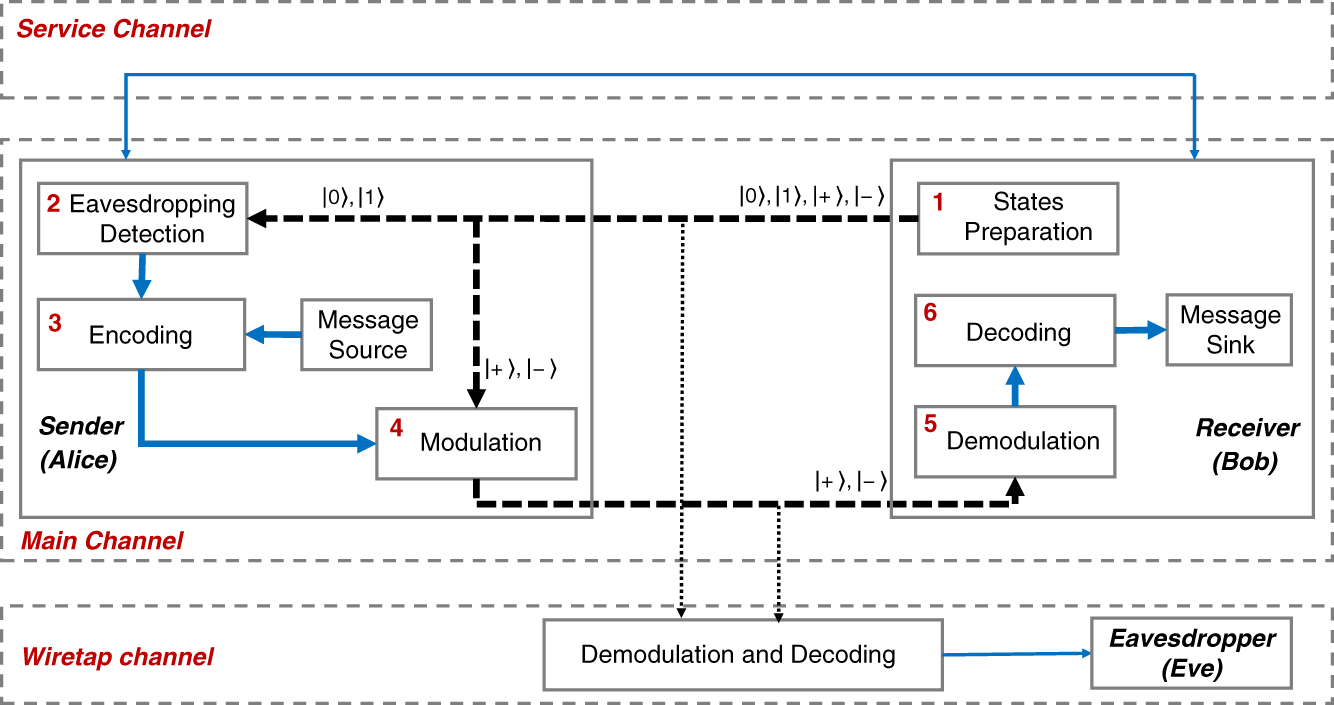
\includegraphics[height=1.0in, width=1.9in, viewport=0 0 1334 705,clip]{Figures/Illustration-of-the-proposed_protocol-for-QDC.png}
%		\caption{\tiny{\textrm{Illustration of the proposed protocol for QDC.}}}%The main channel and wiretap channel are discrete and memoryless. The service channel is a classical authenticated noiseless public channel, which transmits only the associated auxiliary data. The blue lines are classical, while qubits are transmitted over the black dotted lines
%		\label{Fig:Illustration-of-the-proposed_protocol-for-QDC}
                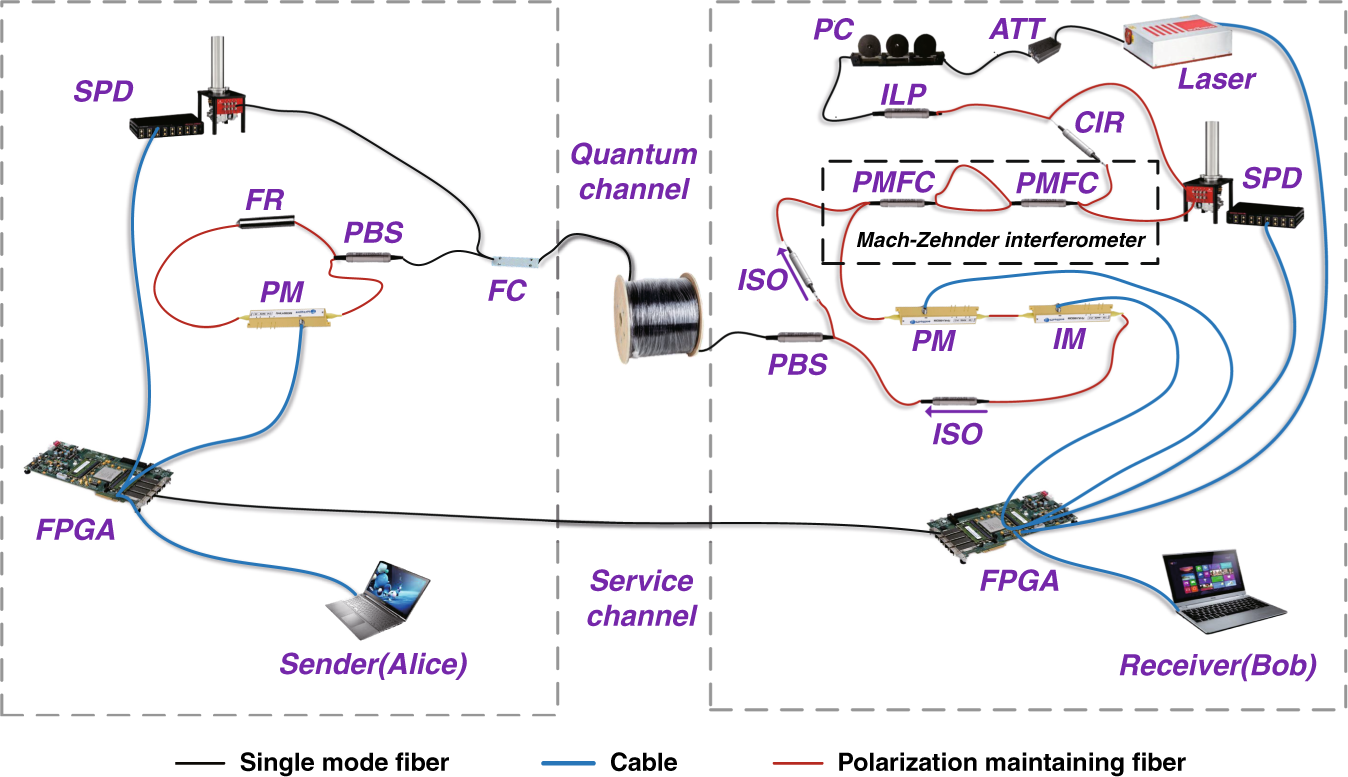
\includegraphics[height=1.0in, width=1.9in, viewport=0 0 1348 777,clip]{Figures/Illustration-of-experiment-setup-for-QDC.png}
%		\caption{\tiny{\textrm{Illustration of experiment setup for QDC.}}}%Laser: 1550 nm with pulse-repetition frequency 50 MHz; FPGA field programmable gate array, ATT attenuator, PC polarization controller, ILP in-line polarizer, CIR optical circulator, PBS polarization beam splitter, FC 90:10 filter coupler, PMFC polarization maintaining filter coupler, PM phase modulator, IM intensity modulator with extinction ratio of 45.1 dB, ISO isolator, FR 90 degree Faraday rotator, SPD superconducting nanowire single-photon detector with over 85% detection efficiency, 50 Hz dark count rate and 15 ns reset time. The asymmetric Mach-Zehnder interferometer consists of two PMFC, and the delay length is about 2 m
		\caption{\tiny{\textrm{Illustration of the proposed protocol and the experiment setup for QDC.}}}
		\label{Fig:Illustration-of-experiment-setup-for-QDC}
    \end{figure}
    \vskip -10pt
		    与传统量子密钥分发后再进行经典加密通信不同,它可直接传递机密信息
\end{frame}

\begin{frame}
    \frametitle{量子直接通信原理}
    \begin{itemize}
        \item 基于量子纠缠或量子叠加原理,对一个粒子的操作会瞬间影响另一个粒子的状态\\
		{\fontsize{7.5pt}{5.2pt}\selectfont{利用纠缠态的量子比特,实现信息的直接传输}}
        \item 发送方通过对本地量子比特进行操作编码信息,接收方通过测量对应的纠缠量子比特来解码信息
    \end{itemize}
    \begin{figure}
        \centering
                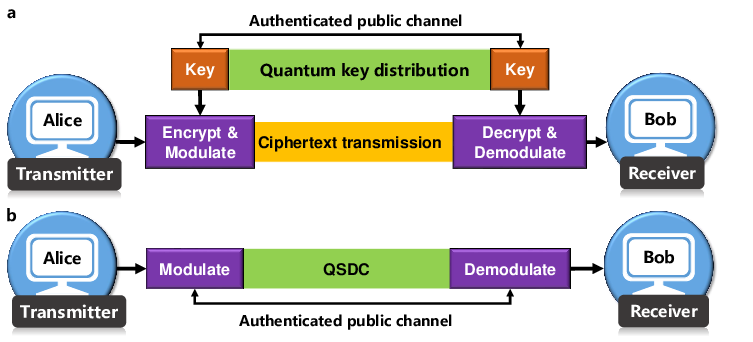
\includegraphics[height=1.5in, width=3.6in, viewport=0 0 250 112,clip]{Figures/Secure-communication-frameworks_Twin-channel-architecture_Single-channel-architecture.png}
		\caption{\tiny{\textrm{Secure communication frameworks: (a)~Twin-channel-architecture, (b)~Single channel architecture.}}}%Secure communication frameworks. a: Twin-channel architecture. b: Single-channel architecture. QSDC: Quantum secure direct communication. Note that QKD uses an authenticated public channel for base sifting and post-processing, while QSDC uses this channel for eavesdropping detection and error correction.
		\label{Fig:Secure-communication-frameworks_Twin-channel-architecture_Single-channel-architecture}
%                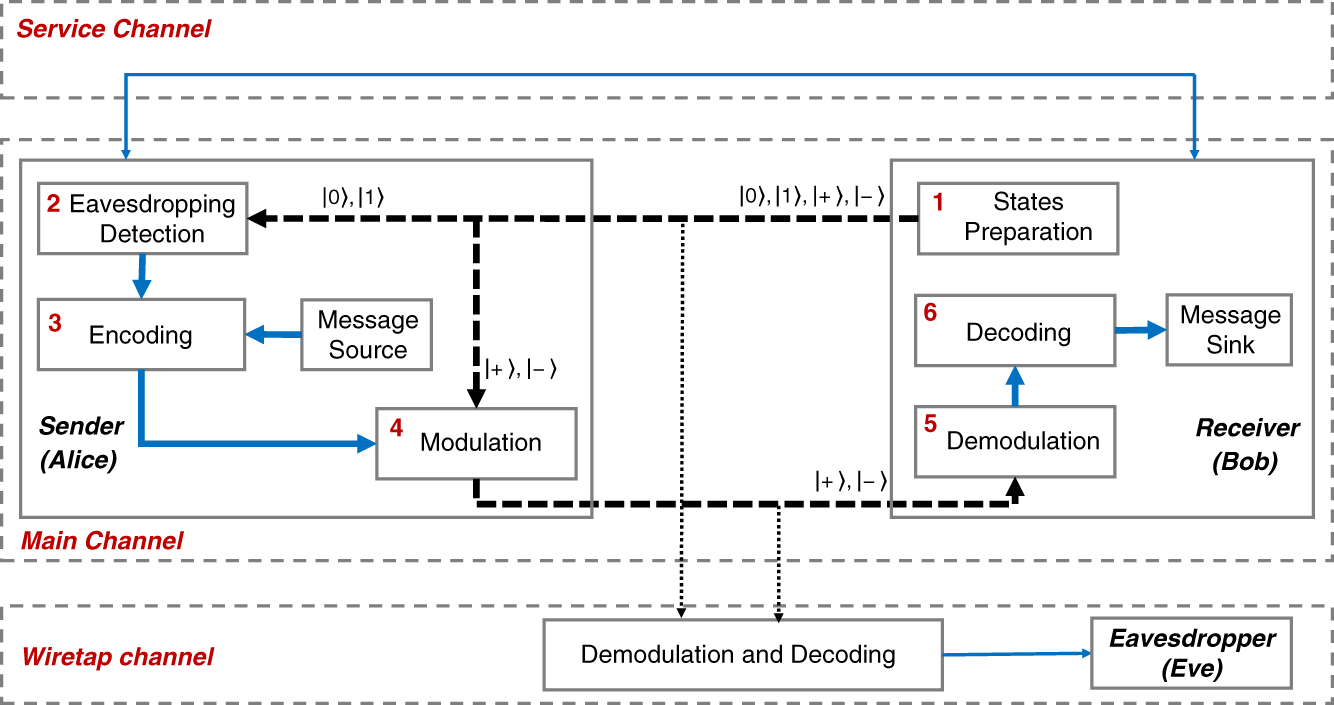
\includegraphics[height=1.5in, width=3.0in, viewport=0 0 1334 705,clip]{Figures/Illustration-of-the-proposed_protocol-for-QDC.png}
%		\caption{\tiny{\textrm{Illustration of the proposed protocol for QDC.}}}%The main channel and wiretap channel are discrete and memoryless. The service channel is a classical authenticated noiseless public channel, which transmits only the associated auxiliary data. The blue lines are classical, while qubits are transmitted over the black dotted lines
%		\label{Fig:Illustration-of-the-proposed_protocol-for-QDC}
%                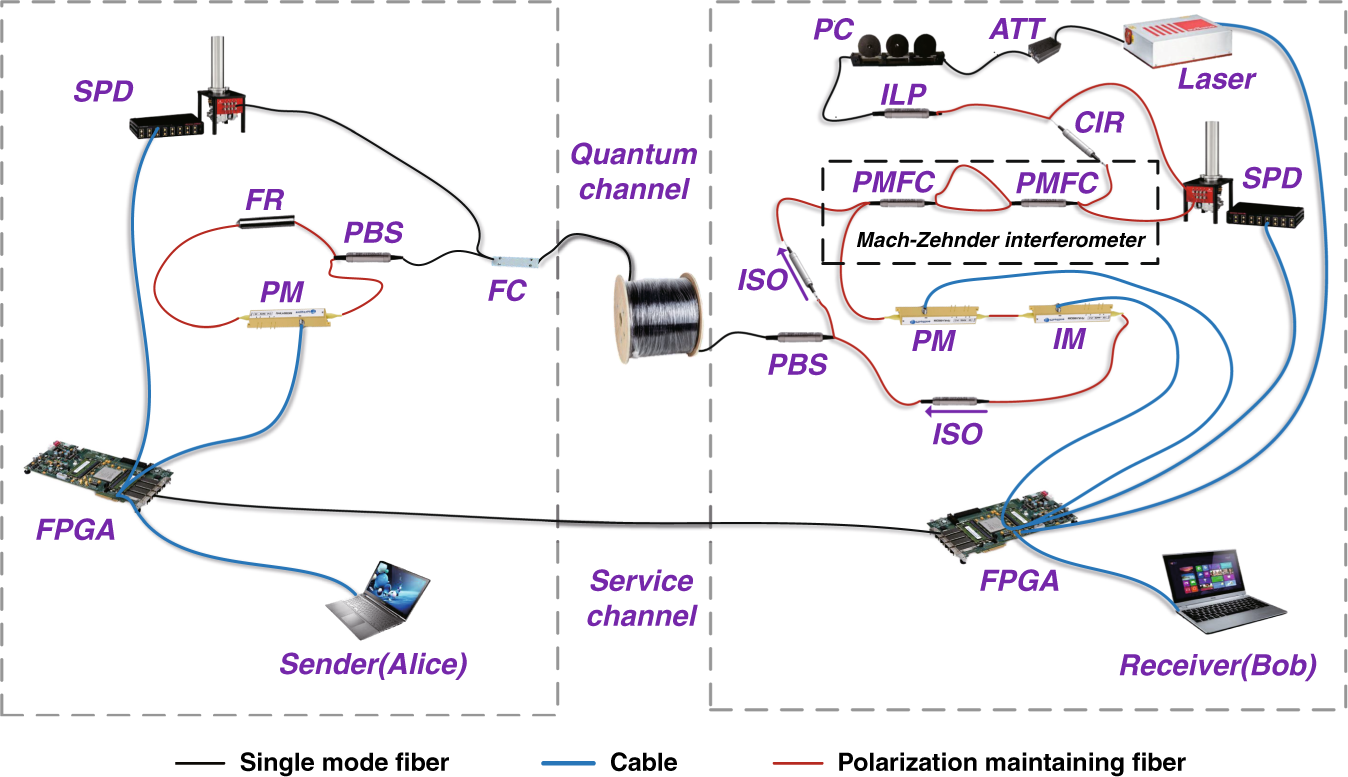
\includegraphics[height=1.5in, width=3.0in, viewport=0 0 1348 777,clip]{Figures/Illustration-of-experiment-setup-for-QDC.jpg}
%		\caption{\tiny{\textrm{Illustration of experiment setup for QDC.}}}%Laser: 1550 nm with pulse-repetition frequency 50 MHz; FPGA field programmable gate array, ATT attenuator, PC polarization controller, ILP in-line polarizer, CIR optical circulator, PBS polarization beam splitter, FC 90:10 filter coupler, PMFC polarization maintaining filter coupler, PM phase modulator, IM intensity modulator with extinction ratio of 45.1 dB, ISO isolator, FR 90 degree Faraday rotator, SPD superconducting nanowire single-photon detector with over 85% detection efficiency, 50 Hz dark count rate and 15 ns reset time. The asymmetric Mach-Zehnder interferometer consists of two PMFC, and the delay length is about 2 m
%		\label{Fig:Illustration-of-experiment-setup-for-QDC}
    \end{figure}
\end{frame}

\begin{frame}
    \frametitle{量子直接通信的优势与挑战}
    \textcolor{red}{优势}:
    \begin{itemize}
	    \item \textcolor{blue}{安全性更高}:~量子力学原理使得任何窃听行为都会改变量子态,被通信双方察觉
	    \item \textcolor{blue}{实时性更强}:~可直接传输信息,无须%像传统量子通信那样
		先进行密钥分发,提高了通信效率
    \end{itemize}

    \textcolor{red}{挑战}:
    \begin{itemize}
        \item 距离限制:~量子态易受环境干扰,导致通信距离受限\\
		{\fontsize{7.5pt}{5.2pt}\selectfont{目前难以实现长距离的直接量子通信}}
        \item 技术复杂度:~对量子态的制备、操控和测量要求高\\
		{\fontsize{7.5pt}{5.2pt}\selectfont{技术实现难度大}}
    \end{itemize}
%    \begin{alertblock}{应对方向}
%        研究人员正在探索量子中继器等技术来延长通信距离,同时不断改进量子操控技术以降低复杂度。
%    \end{alertblock}
\end{frame}

\begin{frame}
    \frametitle{相干中继}
        相干中继:~为解决量子通信中信号传输距离受限问题而提出的一种技术方案\\
	{\fontsize{7.5pt}{5.2pt}\selectfont{在量子信号传输过程中,能有效延长量子态的传输距离,同时保持量子态的相干性}}
    \begin{figure}
        \centering
                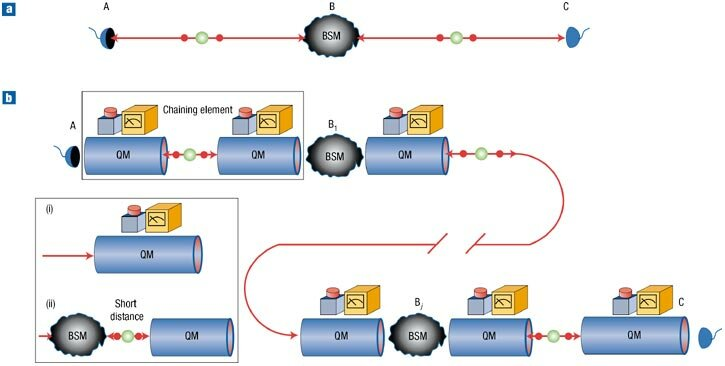
\includegraphics[height=1.8in, width=4.0in, viewport=0 0 725 366,clip]{Figures/Quantum-networksa-Quantum_relay-Entanglement-resources-Quantum_repeater.jpeg}
		\caption{\tiny{\textrm{Quantum networks. Quantum relay and Quantum repeater.}}}%Quantum networks.a, Quantum relay. Entanglement resources and quantum channels joined by means of a BSM, where the entanglement of photons A–B and B–C is swapped to A–C. b, Quantum repeater. An entanglement resource and quantum memories (QM) provide a chaining element that can be concatenated for longer quantum-communication distances, where B1 and Bj denote the connecting BSM links in the repeater chain. The inset illustrates the difference between a 'heralded QM', (i), and a possible modification for a QM without heralding, (ii).}}}
		\label{Fig:Quantum-networksa-Quantum_relay-Entanglement-resources-Quantum_repeater}
    \end{figure}
\end{frame}

\begin{frame}
    \frametitle{相干中继的实现和应用}
    \begin{itemize}
	    \item \textcolor{blue}{量子存储}:~首先要对接收到的量子信号进行存储\\
		    {\fontsize{7.5pt}{5.2pt}\selectfont{利用量子存储器将量子态暂时保存下来,避免信号在传输过程中因损耗而丢失}}
	    \item \textcolor{blue}{纠缠交换}:~通过纠缠交换技术,将不同分段的量子纠缠进行连接和扩展\\
		    {\fontsize{7.5pt}{5.2pt}\selectfont{例如,将相邻两个中继节点之间的纠缠态延伸到更远的距离,使得量子信息能够跨越更长的距离进行传输}}
	    \item \textcolor{blue}{量子纠错}:~在存储和纠缠交换过程中,量子态可能会受到噪声和干扰的影响而发生错误\\
		    {\fontsize{7.5pt}{5.2pt}\selectfont{利用量子纠错编码对错误进行检测和纠正,确保量子态的准确性和相干性}}
    \end{itemize}
   % 相干中继续的远景
    \begin{itemize}
	    \item \textcolor{magenta}{长距离量子通信}:~克服量子信号在光纤等传输介质中的衰减问题,实现洲际甚至全球范围的量子通信\\
		{\fontsize{7.5pt}{5.2pt}\selectfont{为构建全球化的量子通信网络提供可能}}
	\item \textcolor{magenta}{量子互联网}:~作为量子互联网的关键组成部分,相干中继有助于连接不同地区的量子节点\\
		{\fontsize{7.5pt}{5.2pt}\selectfont{实现量子信息在网络中的高效传输和共享,推动量子互联网的发展}}
    \end{itemize}
\end{frame}

\begin{frame}
    \frametitle{中国的量子互联网基建}
    \begin{figure}
        \centering
                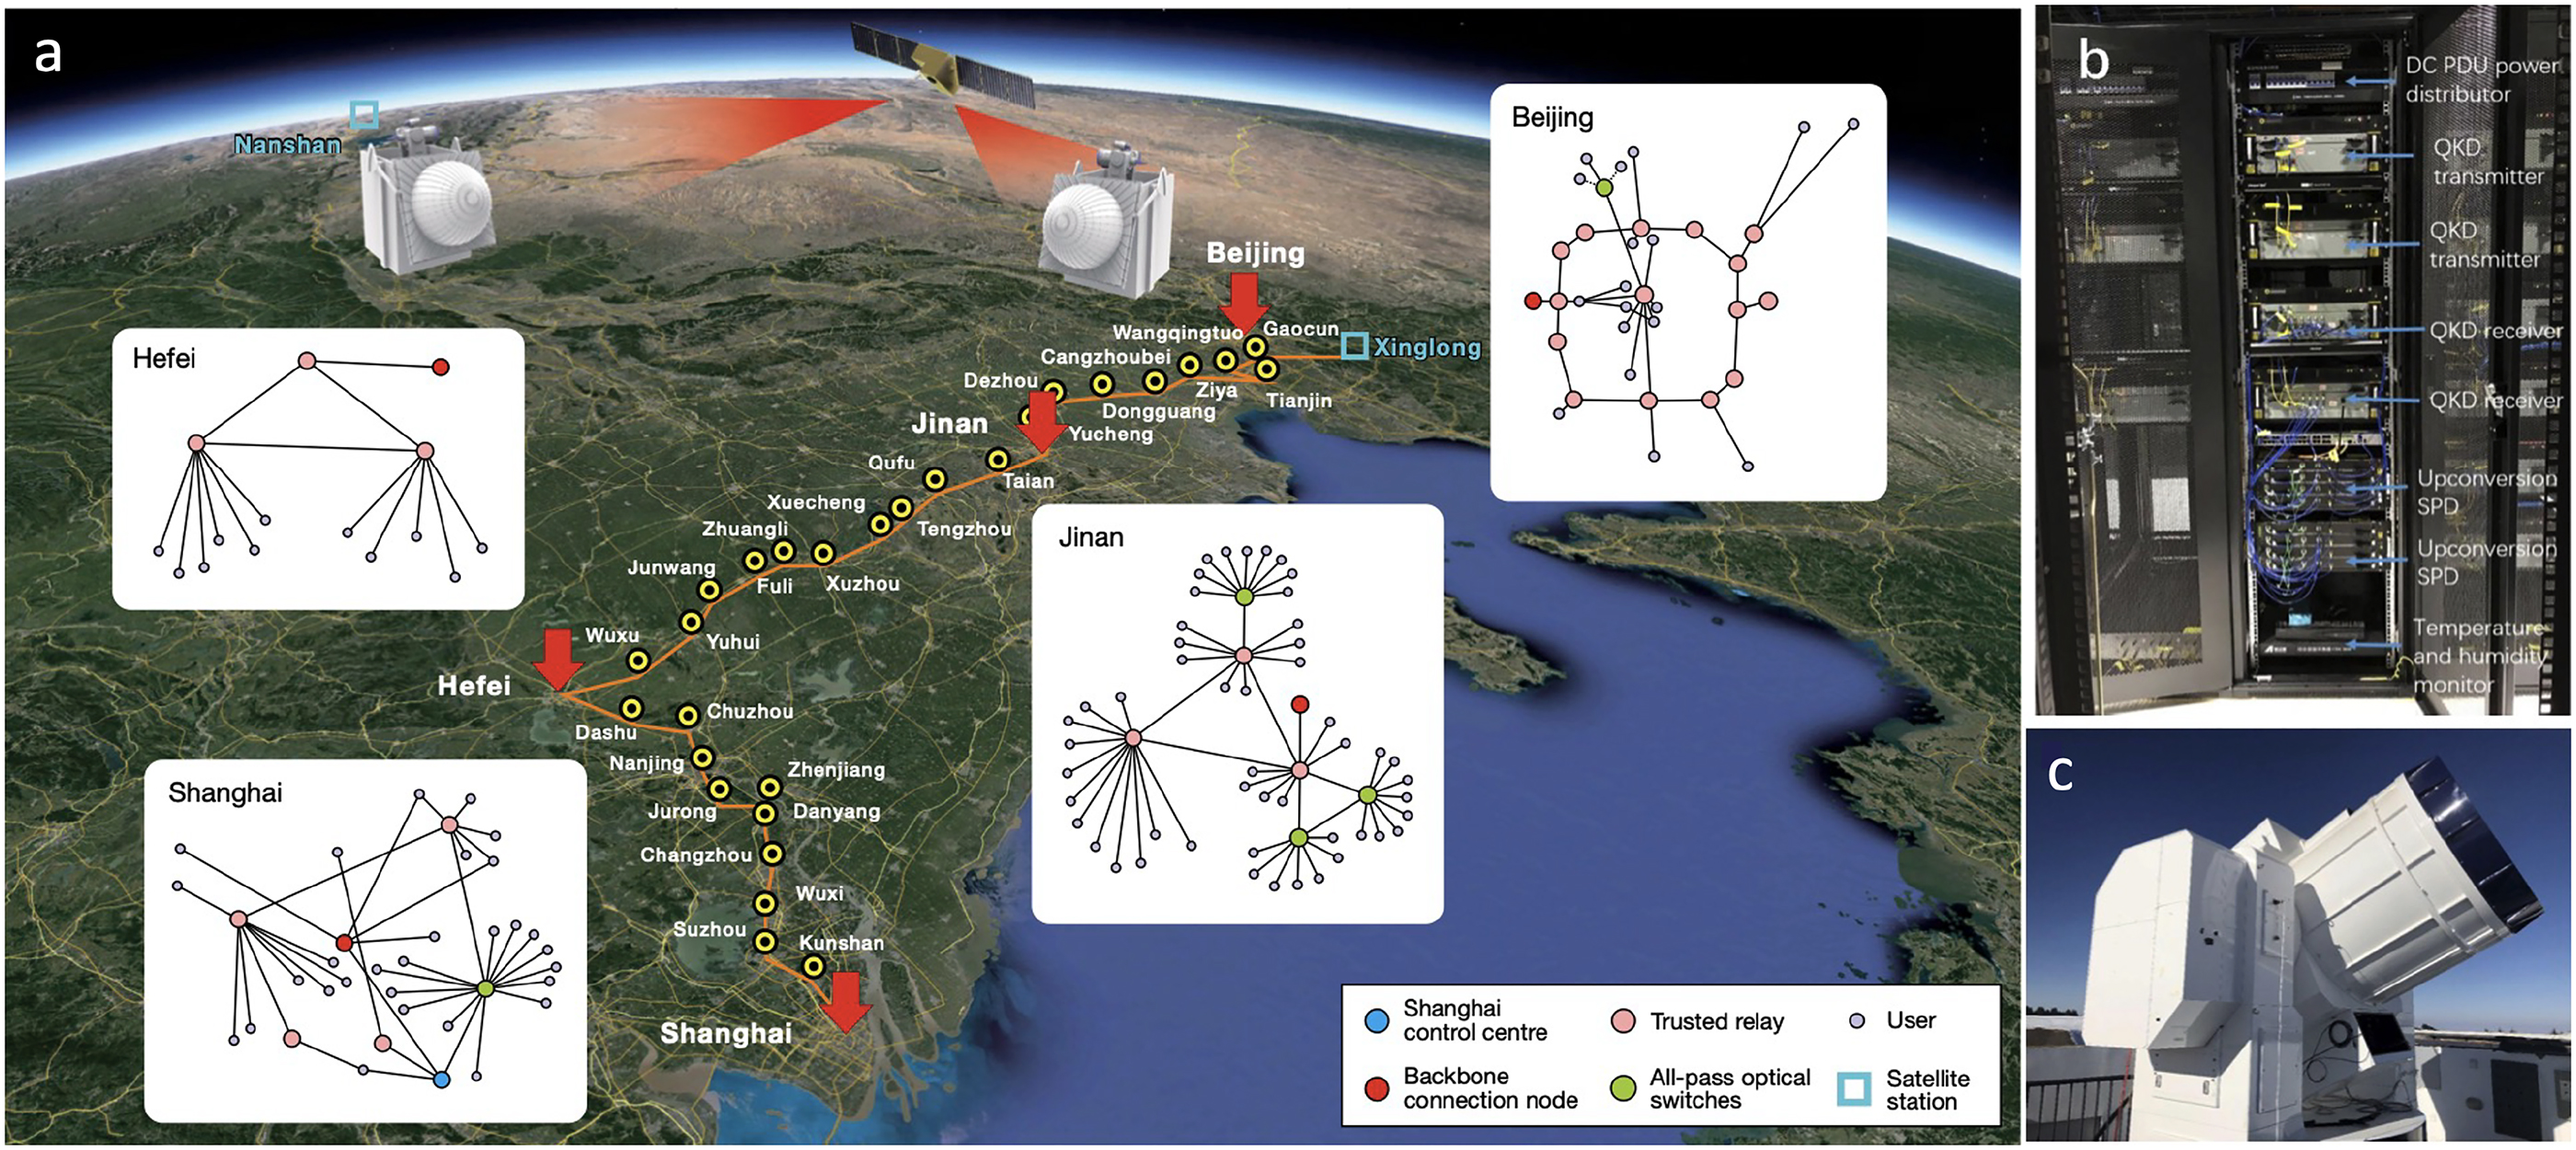
\includegraphics[height=1.9in, width=4.0in, viewport=0 0 525 230,clip]{Figures/Overview-of-the-integrated-space-to-ground-quantum_network-in-China.jpg}
		\caption{\tiny{\textrm{Overview of the integrated space to ground quantum network in China.}}}
		\label{Fig:Overview-of-the integrated-space-to-ground-quantum_network-in-China}
    \end{figure}
\end{frame}

% 量子加密部分
%\section{量子加密}
\begin{frame}
    \frametitle{量子加密}
     利用量子力学原理和特性对信息实施加密:
    %    结合量子通信和传统加密技术,量子相干态为加密提供了新的手段
    \begin{figure}
        \centering
                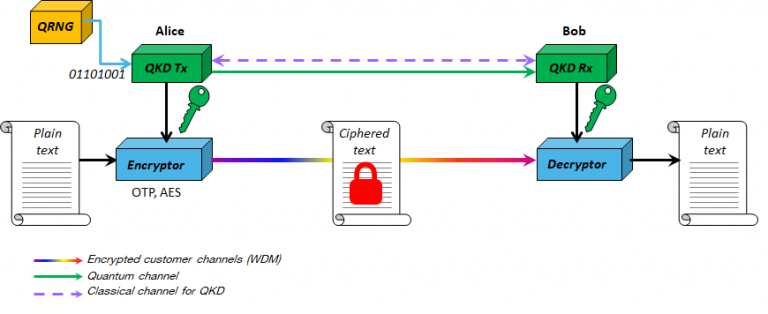
\includegraphics[height=0.9in, width=2.1in, viewport=0 0 568 235,clip]{Figures/Symmetric_encryption-with-quantum_devices.png}
		\caption{\tiny{\textrm{A schematic diagram of symmetric encryption with quantum devices.}}}
		\label{Fig:Symmetric_encryption-with-quantum_devices}
%                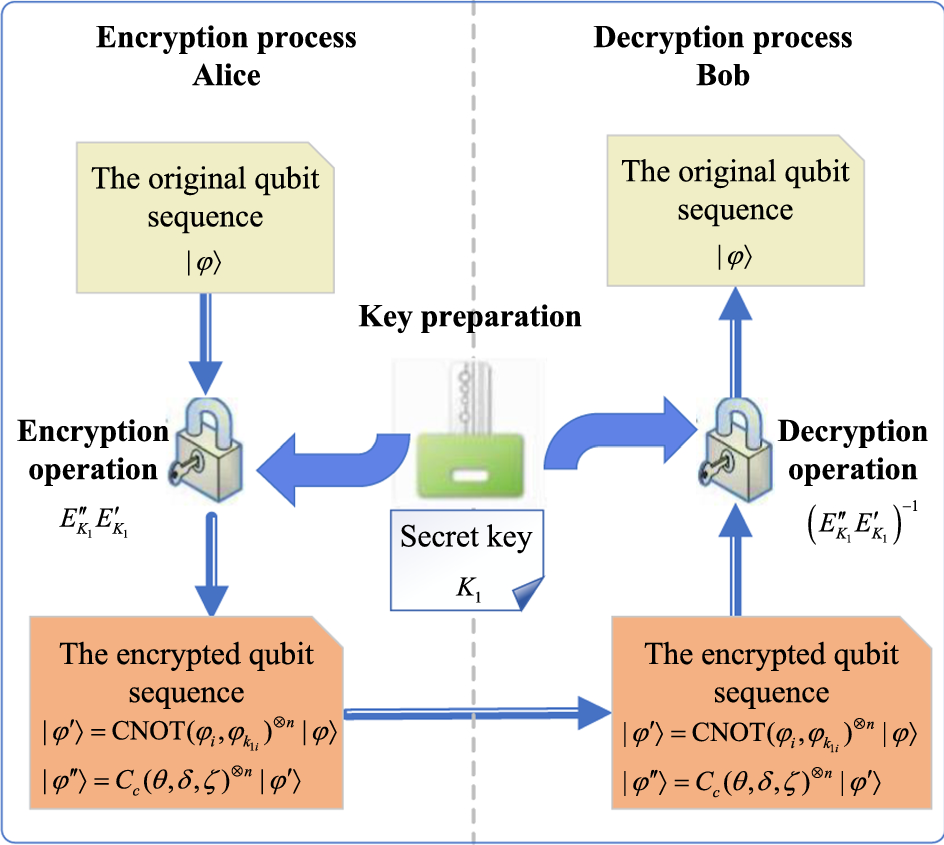
\includegraphics[height=2.0in, width=2.5in, viewport=0 0 944 845,clip]{Figures/Schematic-diagram-of-Quantum_Encryption_Algorithms.png}
%		\caption{\tiny{\textrm{Schematic diagram of Quantum Encryption Algorithms.}}}
%		\label{Fig:Schematic-diagram-of-Quantum_Encryption_Algorithms}
    \end{figure}
    \vskip -10pt
%\end{frame}

%\begin{frame}
%    \frametitle{量子加密的优势}
    \textcolor{blue}{量子加密的优势}
    \begin{itemize}
	    \item \textcolor{red}{无条件安全性}:~基于量子物理原理,无法被破解\\
		    {\fontsize{7.5pt}{5.2pt}\selectfont{\textcolor{blue}{量子相干态的稳定性保证了加密的安全性}}}
	    \item \textcolor{red}{抗干扰能力}:~对外部干扰有较强的抵抗能力
    \end{itemize}
    \begin{exampleblock}{应用场景}
        金融、军事、政府等对信息安全要求极高的领域
    \end{exampleblock}
\end{frame}

% 总结部分
%\section{总结}
%\begin{frame}
%    \frametitle{总结}
%    \begin{itemize}
%        \item 量子相干态是量子计算、量子通信和量子加密的基础
%        \item 量子计算机基于量子比特、叠加原理、纠缠原理和量子门操作实现强大的计算能力。
%        \item 激光冷却与囚禁、约瑟夫森结、量子点等技术为生成量子态提供了有效手段。
%        \item 低温环境控制、电磁屏蔽和量子纠错码等方法有助于保持量子态的稳定性。
%        \item 直接量子通信是一种具有高安全性和实时性的量子通信方式,但面临距离和技术复杂度挑战。
%        \item 量子隐形传态利用量子纠缠实现量子态信息传输,在量子通信网络、量子计算和量子加密等领域有重要应用。
%        \item 相干中继通过量子存储、纠缠交换和量子纠错等技术,有效延长量子信号传输距离并保持相干性,应用于长距离量子通信和量子互联网。
%        \item 量子计算、量子通信和量子加密是量子信息技术的重要组成部分。
%        \item 它们将为未来的信息安全和计算能力带来革命性的变化。
%    \end{itemize}
%    \begin{block}{展望}
%        随着技术的不断发展,量子技术将在更多领域得到应用。
%    \end{block}
%\end{frame}
